\documentclass[11pt,a4paper]{article}
\usepackage[margin=2.4cm,headheight=14pt]{geometry}
\usepackage{fontspec}
\usepackage{amsmath,amssymb}
\usepackage{unicode-math}
\setmainfont{Latin Modern Roman}
\setsansfont{Latin Modern Sans}
\setmonofont{Latin Modern Mono}[Scale=0.95]
\setmathfont{Latin Modern Math}
\usepackage{microtype}
\usepackage{graphicx}
\usepackage{longtable,booktabs,array,tabularx}
\usepackage{caption}
\captionsetup{font=small,labelfont=bf,margin=0.4cm}
\usepackage{float}
\usepackage{enumitem}
\setlist{itemsep=2pt,topsep=4pt}
\usepackage{listings}
\lstset{basicstyle=\ttfamily\footnotesize,breaklines=true,columns=fullflexible,frame=single,framerule=0.3pt}
\usepackage{xcolor}
\definecolor{accent}{HTML}{2A78D6}
\definecolor{linkblue}{HTML}{1F4E9A}
\usepackage{tikz}
\usetikzlibrary{positioning,arrows.meta}
\usepackage[hyphens]{xurl}
\usepackage[colorlinks=true,linkcolor=linkblue,urlcolor=linkblue,citecolor=linkblue,bookmarksnumbered=true,pdfusetitle]{hyperref}
\usepackage{fancyhdr}
\pagestyle{fancy}\fancyhf{}
\fancyhead[L]{\small\itshape Quantitative residual-risk validation for SOTIF}
\fancyhead[R]{\small\thepage}
\renewcommand{\headrulewidth}{0.3pt}
\setlength{\parskip}{3pt plus 1pt}
\setlength{\parindent}{0pt}
\setlength{\emergencystretch}{3em}
\newcolumntype{L}[1]{>{\raggedright\arraybackslash\hspace{0pt}}p{#1}}
\newcommand{\own}[1]{\textit{(this report, #1)}}
\newcommand{\synthetic}{\textsuperscript{\textsf{S}}}
\newcommand{\RHB}{R_{\mathrm{HB}}}
\setcounter{tocdepth}{2}

\title{\textbf{Quantitative Residual-Risk Validation for SOTIF}\\[4pt]
\large From acceptance criteria to scenario-based evidence for an L4 automated driving system}
\author{David Feldmann}
\date{26 October 2026}

\begin{document}
\maketitle
\thispagestyle{empty}

\begin{abstract}
This report collects, in one place, the quantitative chain needed to argue that the residual risk of an automated driving system is acceptable under ISO~21448 (SOTIF). It starts from an acceptance criterion, derives validation targets for field operational testing, and shows why those targets become infeasible for an L4 system. It then develops scenario-based residual-risk estimation (exposure, parameter distributions with a Gaussian copula, importance sampling), works through a fully synthetic example with 100 logical and 1{,}000 concrete scenarios for unintended braking, and derives the field data, statistics and safety performance indicators (SPIs) that the argument needs. It closes with a vehicle-level validation strategy for L4, the role of a scenario database, automatic scenario identification, the granularity of ODD tags, arguments for completeness, and how the approach scales from ACC to an urban robotaxi. Every statement taken from the literature carries a pinpoint citation (section, equation, table, page or slide), so the reader can check it at the source.
\end{abstract}

\noindent\textbf{Highlights}
{\small
\begin{itemize}[leftmargin=1.2em]
\item The Annex~C validation target $\tau=-\ln(1-C)/\RHB$ rests on five assumptions that an assessor can attack; each is stated with its source.
\item Counting critical scenario runs is not a risk estimate; only weights $w=f/q$ connect test runs to real-world exposure.
\item In the synthetic example, the Bayesian 95\% bound passes the budget while a Bonferroni bound over 120 estimates fails: the inference method decides the evidence plan.
\item Ignoring parameter dependence changed $P(\text{collision}\mid\text{HB})$ by a factor of 1.06 to 3.2 in the example.
\item Completeness of a scenario concept cannot be proven; it is argued from construction, explained time, saturation, a risk-weighted remainder and operational monitoring.
\end{itemize}
}

\clearpage
\tableofcontents
\clearpage

%=====================================================================
\section{Introduction}
\subsection{Purpose and scope}
The report supports a SOTIF engineer who must build and defend the quantitative part of a residual-risk argument for a Level~4 system. It covers the statistics behind validation targets, scenario-based risk estimation, the data that feeds it, and how the pieces fit into a vehicle-level validation strategy. It does not cover ISO~26262 hardware metrics or cybersecurity.

\subsection{How sources are cited}
Citations give the location inside the source in square brackets, for example \cite[Sec.~IV-B, Eq.~(1)]{putze2023} or \cite[p.~3, Eq.~2]{kalra2016}. Every location was checked twice against the source texts in October 2026, the second time by verbatim quotation. Four conventions apply:
\begin{itemize}
\item \textbf{ISO 21448.} All references to ISO~21448 were checked directly against ISO~21448:2022(E), first edition 2022-06, and give clause, formula, figure or table and the page number as printed in the standard, e.g.\ \cite[C.3, Formula (C.7), p.~137]{iso21448}.
\item \textbf{Other standards.} ISO/TS~5083 and UL~4600 were not available; their clause and page references are taken from the secondary source named in the same citation, e.g.\ ``ISO/TS~5083, p.~146, as cited in \cite[Sec.~I]{betschinske2025}''.
\item \textbf{Location not verified.} Where only the source, not the location, could be checked, the citation says so.
\item \textbf{Own results.} Numbers computed for this report are marked \own{Sec.~x / Fig.~y}. All example data are synthetic, marked \synthetic, and describe no real system. The code that produces them is listed in Appendix~\ref{app:code}.
\end{itemize}

\subsection{Structure}
Section~\ref{sec:framework} summarises the SOTIF framework for quantitative validation. Section~\ref{sec:vt} derives validation targets from acceptance criteria. Section~\ref{sec:scenario} develops scenario-based risk estimation, and Section~\ref{sec:copula} the Gaussian copula for scenario parameters. Section~\ref{sec:example} works through the unintended-braking example. Section~\ref{sec:field} covers field data, statistics and SPIs. Section~\ref{sec:l4} treats the L4 vehicle-level strategy, the scenario database and completeness. Section~\ref{sec:scaling} discusses scaling to ACC and a robotaxi, and Section~\ref{sec:limits} lists limitations.

%=====================================================================
\section{The SOTIF framework for quantitative validation}\label{sec:framework}
ISO~21448 defines the SOTIF as the absence of unreasonable risk due to hazards resulting from functional insufficiencies of the intended functionality or its implementation \cite[3.25, p.~8]{iso21448}. The scenarios of the relevant use cases are classified into four areas: known not hazardous (area~1), known hazardous (area~2), unknown hazardous (area~3) and unknown not hazardous (area~4); the goal is to reduce areas~2 and~3 to an acceptable level, area~3 through the V\&V strategy of Clauses~9 and~11 \cite[4.2.2, Figures~5--6, pp.~12--14]{iso21448}. The standard stresses that the size of the areas represents the number of scenarios, not the risk, and is not measurable \cite[4.2.2, Notes~2--3, p.~14]{iso21448}. The clauses relevant here are:
\begin{itemize}
\item \textbf{Clause~6:} acceptance criteria are specified for the risks associated with each hazardous behaviour \cite[6.5, p.~30]{iso21448}; an acceptance criterion is a ``criterion representing the absence of an unreasonable level of risk'' \cite[3.1, p.~2]{iso21448}.
\item \textbf{Clause~9:} the V\&V strategy, ``including validation targets'', shall consider the ``sufficient coverage of the relevant scenario space'' and a rationale for the selected methods and validation targets \cite[9.1~a)--b), p.~42]{iso21448}. A validation target is a ``value to argue that the acceptance criterion is met'', and more than one validation target can be needed for one acceptance criterion \cite[3.33 and Note~3, p.~10]{iso21448}.
\item \textbf{Clause~10:} known hazardous scenarios are not unreasonable if their probability of causing hazardous behaviour complies with the validation targets and no known scenario leads to unreasonable risk for specific road users \cite[10.7, pp.~49--50]{iso21448}.
\item \textbf{Clause~11:} ``the validation results shall demonstrate that the residual risk from unknown hazardous scenarios meets the acceptance criteria with sufficient confidence'' \cite[11.1, p.~50]{iso21448}; Table~11 lists the methods, including fleet tests, simulation of random scenario sequences, sensitivity analysis and scenario exploration in the real world \cite[11.3, Table~11, p.~51]{iso21448}.
\item \textbf{Clause~12:} the evaluation asks whether the V\&V strategy covers all known hazardous scenarios and argues that the residual risk from unknown ones meets the acceptance criteria with sufficient confidence \cite[12.3~c), p.~54]{iso21448}.
\item \textbf{Clause~13:} a field monitoring process shall be defined before release and executed during operation \cite[13.1, p.~55]{iso21448}.
\item \textbf{Annex~C:} guidance on V\&V, from deriving validation targets (C.2) to statistics (C.3), scenario parameterisation and sampling (C.5) and reductions of testing (C.6) \cite[C.1, pp.~125--126]{iso21448}.
\end{itemize}
Acceptance criteria can be justified by GAMAB/GAME, a positive risk balance, ALARP or MEM, alone or in combination \cite[6.5, pp.~30--31]{iso21448}; Betschinske et al.\ give the same list \cite[Sec.~III-B, item~2]{betschinske2025}. A secondary summary of the clauses is in \cite[Sec.~2.1, pp.~6--10]{schaller2026}.

ISO~21448 also defines a \emph{vehicle-level SOTIF strategy} (VLSS): a set of vehicle-level \emph{requirements} for the intended functionality, such as transitions to degraded states on ODD exit \cite[3.34, p.~10; D.1, p.~159]{iso21448}. The VLSS is the overarching specification and is itself verified according to the V\&V strategy of Clause~9 \cite[D.1, p.~159]{iso21448}. This report therefore calls the test plan the \emph{vehicle-level V\&V strategy}, not the VLSS.

For L4 systems, ISO~21448 is complemented by:
\begin{itemize}
\item \textbf{ISO/TS~5083}, the ADS-level standard (positive risk balance is already one of the rationales of ISO~21448 6.5). Betschinske et al.\ quote its statement that, for L3, ``a similar amount of real-world test driving as for state-of-the-art L2 systems'' seems appropriate (ISO/TS~5083, p.~146, as cited in \cite[Sec.~I]{betschinske2025}), and argue that carrying the L2 derivation to higher levels gives infeasible targets \cite[Sec.~I]{betschinske2025}.
\item \textbf{ANSI/UL~4600}, which defines safety performance indicators (Sec.~\ref{sec:spi}) (UL~4600 Ch.~16, as cited in \cite[Sec.~2]{ratiu2024} and \cite[slide~12]{koopman2022}).
\item \textbf{The UNECE NATM multi-pillar approach} (audit, simulation, track, real-world testing, in-service monitoring; ECE/TRANS/WP.29/2021/61), on which Commission Implementing Regulation (EU)~2022/1426 builds \cite[web article, no sections]{siemensnatm}.
\end{itemize}

%=====================================================================
\section{From acceptance criterion to validation target}\label{sec:vt}
\subsection{Decomposition of the acceptance criterion}
ISO~21448 decomposes the acceptance criterion $A_H$ for a harm $H$, ``assuming that a hazardous behaviour does not lead always to a harm'', as
\begin{equation}
A_H = \RHB \cdot P(E\mid \mathrm{HB}) \cdot P(\bar C\mid E)\cdot P(S\mid \bar C)
\label{eq:annexc}
\end{equation}
\cite[C.2.1, Formula~(C.1), p.~127]{iso21448}; the same formula is discussed in \cite[Sec.~IV-B(a), Eq.~(1)]{putze2023} and \cite[Sec.~V, Eqs.~(6)--(7)]{betschinske2025}. The standard writes $P_{E|HB}$, $P_{C|E}$ and $P_{S|C}$: $P_{C|E}$ is ``the probability that the hazardous behaviour is not controllable'', and $P_{S|C}$ the probability of a degree of severity ``assuming that the controllability action was not successful'' \cite[C.2.1, p.~126]{iso21448}; this report writes $\bar C$ to make that explicit. Solving for $\RHB$ gives the tolerable hazardous-behaviour rate \cite[C.2.1, Formula~(C.2), p.~127]{iso21448}. The standard's example: $A_H=10^{-8}$/h, $P_{C|E}=10\%$, $P_{S|C}=1\%$, $P_{E|HB}=5\%$ give $\RHB=2\times10^{-4}$/h, and 5{,}000~h without hazardous behaviour show the criterion met with 63\% confidence \cite[C.2.1, Formula~(C.3) and Example, p.~127]{iso21448}.

Putze et al.\ raise three objections \cite[Sec.~IV-B(b)]{putze2023}; the standard's own wording, given after each, answers them only in part:
\begin{enumerate}
\item A correct chain-rule decomposition needs further conditioning, e.g.\ $P(S\mid \bar C, E, \mathrm{HB})$ instead of $P(S\mid\bar C)$. The standard notes that the product of simple probabilities applies when the triggering conditions are independent of the exposure \cite[C.2.1, Note~5, p.~127]{iso21448}.
\item Annex~C.2.1 omits the aggregation over several hazardous behaviours leading to the same harm, without flagging this as a simplification. The standard links every hazardous behaviour to its own acceptance criterion and derives $A_H$ ``from original acceptance criteria in combination with safety margin'' \cite[C.2.1, p.~126]{iso21448}, but does not say how the original criterion is split.
\item Field-data quantities are not system-independent: exposure depends on route planning and the ODD; their example is the probability of a truck in front \cite[Sec.~IV-B(c)]{putze2023}. The standard says the parameters ``can be checked for consistency'' with the ISO~26262 HARA \cite[C.2.1, Note~4, p.~127]{iso21448}.
\end{enumerate}
They therefore bound the harm probability over triples of triggering condition $T$, behaviour $B$ and event $E$:
\begin{equation}
P(H) \le \sum_{T,B,E} P(T)\,P(B\mid T)\,P(E\mid B,T)\,P(H\mid E,B,T)
\label{eq:bonf}
\end{equation}
\cite[Sec.~IV-B(b), Eq.~(2); severity-stratified form Eq.~(3)]{putze2023}, and conclude that ``it is not sufficient to derive a single validation target'' \cite[Sec.~IV-B(b), last paragraph]{putze2023}.

\subsection{The zero-failure test}
Assuming that incidents have a Poisson distribution, ISO~21448 gives the driving $\tau$ without potentially hazardous behaviour needed to show an incident rate $\le A_H$ ``with a confidence $\alpha$'' as $\tau=-\ln(1-\alpha)/A_H$ \cite[C.3, Example~3 and Formula~(C.7), p.~137]{iso21448}, taken from Littlewood and Wright \cite{littlewood1997}. Applied to the tolerable rate of Eq.~\eqref{eq:annexc}, as in the standard's own example \cite[C.2.1, p.~127]{iso21448} and in \cite[Sec.~IV-B(a)]{putze2023}, and writing $C$ for the confidence:
\begin{equation}
\tau = \frac{-\ln(1-C)}{\RHB}
\label{eq:tau}
\end{equation}
For $C\approx0.63$, $\tau = 1/A_H$ \cite[C.3, Note~2, p.~137]{iso21448}. Equation~\eqref{eq:tau} gives confidence $C$ about $\RHB$ only; it transfers to $A_H$ only if the factors of Eq.~\eqref{eq:annexc} are known exactly. With estimated factors, use their upper bounds and split the confidence, $\tau=-\ln(1-C_1)\,\prod P^{U}/A_H$ at overall confidence $\ge C_1+C_2-1$, as Betschinske et al.\ do for a decomposed hazardous behaviour \cite[Sec.~V, Eq.~(9)]{betschinske2025}. The standard adds that $\tau$ ``can be quite large and therefore not practical in some cases'' and can be lessened with expert knowledge and MIL, SIL and HIL kilometres \cite[C.3, p.~137]{iso21448}; Betschinske et al.\ call it the real-world driving requirement \cite[Sec.~III-C, item~5, Eq.~(5)]{betschinske2025}. Betschinske et al.\ write the test as $H_0\!: R > A_H$ against $H_1\!: R\le A_H$ with the type-I error bound $P(X\le k)\le\alpha$, $\lambda = A_H\tau_k$ \cite[Sec.~III-C, Eqs.~(3)--(4)]{betschinske2025}.

\textbf{Notation trap.} In Formula~(C.7) $\alpha$ is the \emph{confidence} \cite[C.3, p.~137]{iso21448}, and Putze et al.\ follow this \cite[Sec.~IV-B(a)]{putze2023}. In C.6.3.2 the same standard writes the confidence as $1-\alpha$, i.e.\ $\alpha$ is an error level \cite[C.6.3.2, Example~1, p.~156]{iso21448}, and Betschinske et al.\ use $\alpha$ as type-I error, so their Eq.~(5) reads $-\ln(\alpha)/A_H$ \cite[Sec.~III-C, Eq.~(5)]{betschinske2025}. This report writes $C$ for confidence throughout.

At $C=0.95$, $-\ln 0.05\approx 3.00$ (the ``rule of three''). Kalra and Paddock use the per-mile form $n=\ln(1-C)/\ln(R)$ with reliability $R=1-F$ \cite[Sec.~1, p.~3, Eq.~2]{kalra2016}. With the US fatality rate of 1.09 per 100 million miles in 2013 \cite[Introduction, p.~2]{kalra2016}, this gives 275 million failure-free miles, or about 12.5 years for 100 vehicles driving 24/7 at 25~mph \cite[Sec.~1, p.~3; Table~1, p.~10]{kalra2016}. Demonstrating a fatality rate 20\% below the human rate with 95\% confidence and 80\% power takes more than 11 billion miles, about 518 years \cite[Sec.~3, p.~8]{kalra2016}.

The standard notes that acceptance criteria are usually very small, e.g.\ $10^{-8}$/h \cite[C.2.1, p.~126]{iso21448}. Schaller et al.\ give the example criterion ``overlooking a car on the other lane is at most $10^{-9}$ per hour'', the order of magnitude used in civil aviation for extremely improbable failure conditions, and call the testing needed to prove it prohibitive \cite[Sec.~5.1, p.~14]{schaller2026}. Equation~\eqref{eq:tau} gives $3.0\times10^{9}$~h, about 342{,}000 vehicle-years of 24/7 operation \own{Sec.~\ref{sec:vt}}.

\subsection{Plans that allow \texorpdfstring{$k$}{k} events}
If the plan allows $k$ events, the pass condition $P(X\le k\mid\lambda)\le 1-C$ is solved by
\begin{equation}
\tau_k = \frac{\lambda_k(C)}{\RHB},\qquad \lambda_k(C)=\tfrac12\,\chi^2_{2(k+1)}(C),
\label{eq:chi2}
\end{equation}
the classical relation between Poisson confidence limits and the $\chi^2$ distribution \cite[location not verified]{garwood1936}. Table~\ref{tab:lambda} gives the factors \own{computed with SciPy}.

\begin{table}[H]
\centering\small
\caption{Factors $\lambda_k(C)$ for plans allowing $k$ events \own{computed}.}
\label{tab:lambda}
\begin{tabular}{lrrrrrr}
\toprule
$C$ \textbackslash{} $k$ & 0 & 1 & 2 & 3 & 4 & 5\\
\midrule
0.90 & 2.303 & 3.890 & 5.322 & 6.681 & 7.994 & 9.275\\
0.95 & 2.996 & 4.744 & 6.296 & 7.754 & 9.154 & 10.513\\
0.99 & 4.605 & 6.638 & 8.406 & 10.045 & 11.605 & 13.108\\
\bottomrule
\end{tabular}
\end{table}

$k$ and $\tau$ must be fixed before testing: under classical hypothesis testing, the test cannot be extended after a failure without inflating the type-I error \cite[Sec.~III-C, item~6]{betschinske2025}. ISO~21448 likewise lists, among what the system owner specifies prior to testing, the validation target as ``stopping rule'' and the ``criterion for restarting distance counter'' \cite[C.3, p.~136]{iso21448}. Raising $C$ from 0.95 to 0.99 multiplies $\tau$ by $\ln 0.01/\ln 0.05 = 1.54$; allowing $k=1$ at $C=0.95$ multiplies it by 1.58 \own{Table~\ref{tab:lambda}}.

\subsection{What a passed test silently assumes}
\begin{enumerate}
\item \textbf{Homogeneous Poisson process}: constant rate and independent events (the Poisson assumption in \cite[Sec.~IV-B(a)]{putze2023}).
\item \textbf{Representative exposure}: the tested mix of conditions equals the deployed mix; the factors in Eq.~\eqref{eq:annexc} are system-dependent \cite[Sec.~IV-B(b)--(c)]{putze2023}.
\item \textbf{Frozen software}: a fix invalidates earlier hours unless carry-over is argued; the standard's example assumes ``sensor and algorithms are fixed during testing and real-world use'' \cite[C.6.3.2, p.~154]{iso21448}, and new unknown hazardous scenarios can arise with algorithm, ODD or driving-policy changes \cite[11.3, Note~1, p.~52]{iso21448}; reusing earlier systems' data is a main validity gap \cite[Sec.~V, RA ``Decomposition of Hazardous Behavior'' and ``Bayesian Statistics'']{betschinske2025}.
\item \textbf{One behaviour per harm}: otherwise rates add, Eq.~\eqref{eq:bonf} \cite[Sec.~IV-B(b)]{putze2023}. Aggregating separately validated terms gives a joint confidence of at least $1-(\alpha_1+\alpha_2)$ \cite[C.6.3.2, Example~1 and footnote~1, p.~156]{iso21448}. (Betschinske et al.\ cite this as ``p.~165'' \cite[Sec.~V, RA ``Decomposition of Hazardous Behavior'']{betschinske2025}; in the printed standard it is on p.~156.)
\item \textbf{Frequentist meaning}: a system exactly at the limit passes with probability at most $1-C$; a posterior statement needs a prior. The flat prior Gamma$(1,0)$ reproduces the base model, Jeffreys' Gamma$(0.5,0)$ lowers the requirement \cite[Sec.~V, RA ``Bayesian Statistics'']{betschinske2025}.
\end{enumerate}

\subsection{Ways to reduce the effort}
The standard itself offers: focusing validation on the most severe modality of a partitioned usage variable \cite[C.6.1, p.~153]{iso21448}; sufficient conditions at component level, e.g.\ $E[\text{collisions}]\le P(D_m>c)\,E[\text{objects}]$ with separately estimated factors \cite[C.6.2, p.~153; C.6.3.2, pp.~154--156]{iso21448}; and redundant, independent channels \cite[C.6.3.3, pp.~156--158]{iso21448}. Betschinske et al.\ review further reduction approaches. Sequential testing (Wald's SPRT) allows optional stopping only if both hypotheses are set at or stricter than the acceptance threshold, $\theta_0,\theta_1\ge\theta_{A_H}$, and gives a reduction only if $\beta>1-c$ with $c=\tfrac{\theta_0}{\theta_1}\alpha^{\theta_0/\theta_1}$ \cite[Sec.~V, RA ``Sequential Testing'', Eqs.~(14)--(15)]{betschinske2025}. Further approaches are decomposition of the hazardous behaviour \cite[Sec.~V, Eqs.~(8)--(9)]{betschinske2025}, high-yield route profiles with importance-sampling correction \cite[Sec.~V, RA ``High Yield Route Profiles'', Fig.~12]{betschinske2025}, extreme value analysis \cite[Sec.~V, RA ``Extreme Value Analysis'', Table~IX]{betschinske2025} and scenario-based testing \cite[Sec.~V, RA ``Scenario Based Testing'', Table~XI]{betschinske2025}. Direct mileage-based validation of upper bounds on harm probability is not feasible for ADS \cite[Sec.~IV-A(b), citing Wachenfeld and Winner]{putze2023}, and a residual dependence on field testing is likely to remain \cite[Sec.~VII]{betschinske2025}.

%=====================================================================
\section{Scenario-based residual risk}\label{sec:scenario}
\subsection{Direction of the calculation}
A HARA is built from the system outward: hazardous behaviour, hazardous event, scenarios. Probability flows the other way: the world produces situations at some rate, and the system responds with a hazardous behaviour or not. For the risk calculation the scenario is the random variable and the behaviour is conditioned on it. Logical scenarios must partition the ODD; overlapping scenarios double-count exposure, and then only the bound \eqref{eq:bonf} holds \cite[Sec.~IV-B(b), Eq.~(2)]{putze2023}.

\subsection{The estimator}
For a severity class $s$ and logical scenarios $\ell$ with exposure $\nu_\ell$ (occurrences or time share per operating hour) and parameter distribution $f_\ell(\theta)$:
\begin{equation}
R_s=\sum_\ell \nu_\ell\,p_{\ell,s},\qquad p_{\ell,s}=\int P(\mathrm{HB}\mid\theta,\ell)\,P(S\ge s\mid\mathrm{HB},\theta,\ell)\,f_\ell(\theta)\,d\theta .
\label{eq:risk}
\end{equation}
De Gelder computes risk in the same spirit, by combining the outcome of virtual simulations with the estimated likelihood of scenarios, and decomposes it into exposure, crash probability and severity \cite[Ch.~1 and Ch.~7, Secs.~7.3.2, 7.3.4, 7.3.5]{degelder2022}. From $N$ concrete runs drawn from a test distribution $q_\ell$, the importance-sampling estimator is
\begin{equation}
\hat p_{\ell,s}=\frac1N\sum_{i=1}^N w_i h_i,\qquad w_i=\frac{f_\ell(\theta_i)}{q_\ell(\theta_i)},\qquad \mathrm{ESS}=\frac{(\sum_i w_i)^2}{\sum_i w_i^2}
\label{eq:is}
\end{equation}
(importance sampling and effective sample size: \cite[Ch.~9]{owen2013}). Kish's ESS depends only on the weights, not on the outcome $h$; for rare-event estimates the relative standard error of $\hat p$, $\widehat{\mathrm{sd}}(w h)/(\sqrt N\,\hat p)$, is the quantity to report (Sec.~\ref{sec:audit}). ISO~21448 describes the same building blocks: parameter distributions determined from naturalistic driving data, e.g.\ by kernel density estimation \cite[C.5, Figures~C.9--C.11, pp.~146--148]{iso21448}, importance sampling that biases the test parameters towards riskier areas \cite[C.5, Figures~C.12--C.14, pp.~149--151]{iso21448}, and a final risk estimate ``based on the simulation results and depending on the acceptance criteria'' \cite[C.5, p.~151]{iso21448}. Zhao et al.\ apply importance sampling with cross-entropy-optimised proposals to lane-change scenarios from naturalistic data and report acceleration factors of about 2{,}000 to 20{,}000 \cite[Abstract]{zhao2017}.

\subsection{Counting critical runs is not a risk estimate}
Figure~\ref{fig:toy} shows why. In a toy cut-in model, a uniform test design puts 5.4\% of its runs in the failure region, while the real-world probability of failure per cut-in is $4.9\times10^{-5}$ \own{Fig.~\ref{fig:toy}\synthetic}. Non-critical runs are evidence too. Falsification and criticality search find triggering conditions (Clause~10), but do not estimate risk unless $q$ is known. Figure~\ref{fig:conv} shows importance sampling converging long before plain Monte Carlo sees its first collision.

\begin{figure}[H]\centering
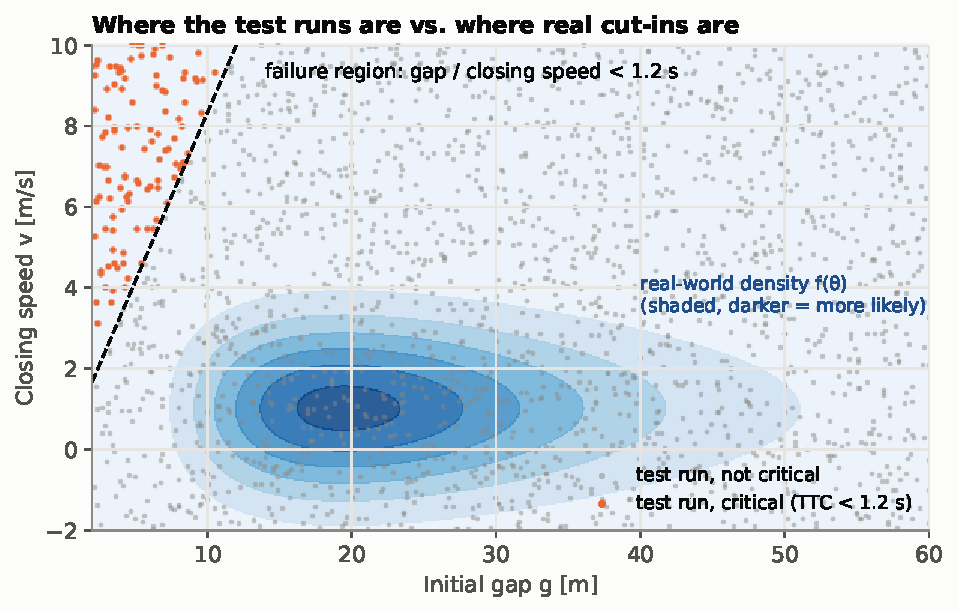
\includegraphics[width=0.86\linewidth]{figures/f01_toy_cutin.pdf}
\caption{Toy cut-in\synthetic: test runs of a uniform design against the real-world density. 5.4\% of runs are critical; the real-world failure probability is $4.9\times10^{-5}$ \own{computed}.}
\label{fig:toy}
\end{figure}
\begin{figure}[H]\centering
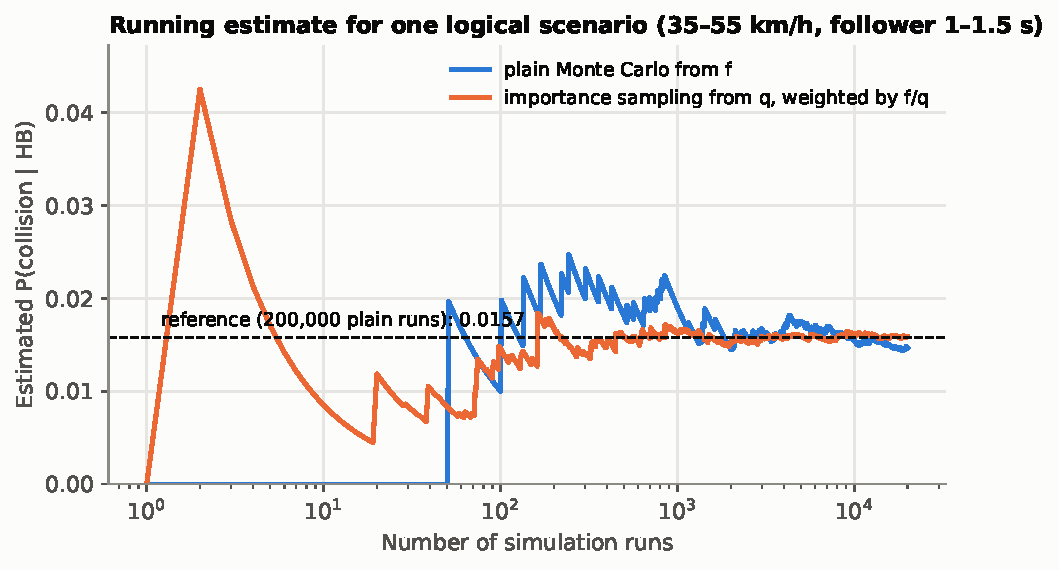
\includegraphics[width=0.86\linewidth]{figures/f02_convergence.pdf}
\caption{Running estimate of $P(\text{collision}\mid\mathrm{HB})$ for one logical scenario\synthetic: plain Monte Carlo versus importance sampling, against a 200{,}000-run reference of 0.0157 \own{computed}.}
\label{fig:conv}
\end{figure}

\subsection{Relation to validation targets}
The single target $\tau$ of Eq.~\eqref{eq:tau} is replaced by one claim with several evidence targets:
\begin{equation}
\sum_\ell \nu_\ell^{U}\,p_{\ell,s}^{U} + R^{U}_{\text{unknown}}\le A_s \quad\text{at confidence } C,\qquad \sum_i (1-C_i)\le 1-C,
\label{eq:claim}
\end{equation}
where superscript $U$ marks upper confidence bounds and the confidence budget is split by Bonferroni's inequality.

\begin{table}[H]\centering\small
\caption{Evidence targets that replace the single field-test target.}
\label{tab:evidence}
\begin{tabular}{L{2.6cm}L{8.3cm}L{3.4cm}}
\toprule
Term & Validation target & Measured in\\\midrule
$\nu_\ell^U$ & enough naturalistic data per scenario class (Poisson bound on counts) & hours of ODD data\\
$f_\ell$ & estimation error of the fitted distribution below a threshold; de Gelder quantifies completeness via the expected approximation error of a KDE \cite[Ch.~3]{degelder2022} & scenario instances\\
$p_\ell^U$ & upper bound per scenario; plain Monte Carlo with zero failures needs $N=3/p^*$ runs, so importance sampling is required & runs, ESS\\
simulation credibility & real-versus-simulated agreement for the same $\theta$; ``how accurately the models represent the real world is part of the safety argument'' \cite[C.1, p.~125]{iso21448}; NATM includes a credibility assessment framework \cite[web article]{siemensnatm} & proving ground, replays\\
$R^U_{\text{unknown}}$ & field driving without unexplained HB, Eq.~\eqref{eq:tau} restricted to what the taxonomy misses & hours\\
\bottomrule
\end{tabular}
\end{table}
Scenario-based testing lacks a direct quantitative link to mileage and an agreed coverage threshold \cite[Sec.~V, RA ``Scenario Based Testing'', Table~XI]{betschinske2025}. It shrinks the field-testing target but does not remove it \cite[Sec.~VII]{betschinske2025}.

\subsection{Parameterising logical scenarios}
\begin{enumerate}
\item Define the scenario type and its parameters, following the logical/concrete distinction of ISO~34502 \cite[location not verified]{iso34502}; ISO~21448 parameterises a lead-braking scenario by $v_{\text{end}}$, $t_{\text{brake}}$ and $\Delta v$ \cite[C.5, Figure~C.10, p.~147]{iso21448}.
\item Keep $\theta$ small (3--6 dimensions) by sensitivity analysis; ISO~21448 asks that parameter selection be argued ``by, for example, sensitivity analysis or statistical analysis'' \cite[11.3, Table~11 Note, p.~51]{iso21448}; Glasmacher et al.\ list parameter sensitivity analysis in simulation as data-driven evidence \cite[Sec.~III-D, Table~I]{glasmacher2024}.
\item Mine instances from drive logs with a scenario tagger \cite[Secs.~III-A--III-C]{guo2023}; each detection gives one $\theta$ sample and one count towards $\nu$.
\item Fit $f_\ell$: marginals plus copula (Sec.~\ref{sec:copula}) or kernel density estimation \cite[Ch.~3 and Ch.~6]{degelder2022}.
\item Estimate $\hat\nu_\ell=n_\ell/T$ with a Poisson or Gamma interval.
\item Check the partition: no instance may belong to two logical scenarios.
\end{enumerate}

\subsection{Where each conditional probability comes from}
\begin{table}[H]\centering\small
\caption{Sources of the terms in Eq.~\eqref{eq:risk}.}
\begin{tabular}{L{2.4cm}L{6.6cm}L{5.4cm}}
\toprule
Quantity & Primary source & Caveat\\\midrule
$\nu_\ell, f_\ell(\theta)$ & own fleet logs; public naturalistic data only if the ODD matches & system-dependent, e.g.\ exposure depends on routing and ODD \cite[Sec.~IV-B(b)--(c)]{putze2023}\\
$P(\mathrm{HB}\mid\theta)$ & simulation with a perception error model learned from labelled field data; runtime monitors flag near-failure situations \cite[Sec.~6.2, pp.~16--17]{schaller2026} & simulation fidelity is limited \cite[Sec.~V, RA ``Simulation-based Testing'']{betschinske2025}\\
$P(\bar C\mid E)$ & for L4: evasion by other road users, via reactive agent models, or 1 & an assumption to justify\\
$P(S\mid\mathrm{HB},\theta)$ & simulated $\Delta v$ and impact angle, then an injury-risk curve, e.g.\ an omni-directional injury model \cite[web page]{waymoinjury} & carry the curve's confidence band\\
\bottomrule
\end{tabular}
\end{table}

%=====================================================================
\section{Gaussian copula for scenario parameters}\label{sec:copula}
\subsection{Definition}
By Sklar's theorem, every joint distribution function can be written as $F(x_1,\dots,x_d)=C\big(F_1(x_1),\dots,F_d(x_d)\big)$ with a copula $C$ \cite[Sec.~2.3]{nelsen2006}. The Gaussian copula is $C_R(u)=\Phi_R\big(\Phi^{-1}(u_1),\dots,\Phi^{-1}(u_d)\big)$. Each scenario parameter keeps its own marginal, and the correlation matrix $R$ alone sets the dependence.

\subsection{Sampling and density}
Sampling: $\varepsilon\sim\mathcal N(0,I)$, $Z=L\varepsilon$ with $R=LL^\top$, $U_i=\Phi(Z_i)$, $X_i=F_i^{-1}(U_i)$. The copula density, needed for the weights in Eq.~\eqref{eq:is}, is
\begin{equation}
c_R(u)=|R|^{-1/2}\exp\!\Big(-\tfrac12 z^\top(R^{-1}-I)z\Big),\quad z=\Phi^{-1}(u),\qquad f(x)=c_R\big(F(x)\big)\prod_i f_i(x_i).
\end{equation}

\begin{figure}[H]\centering
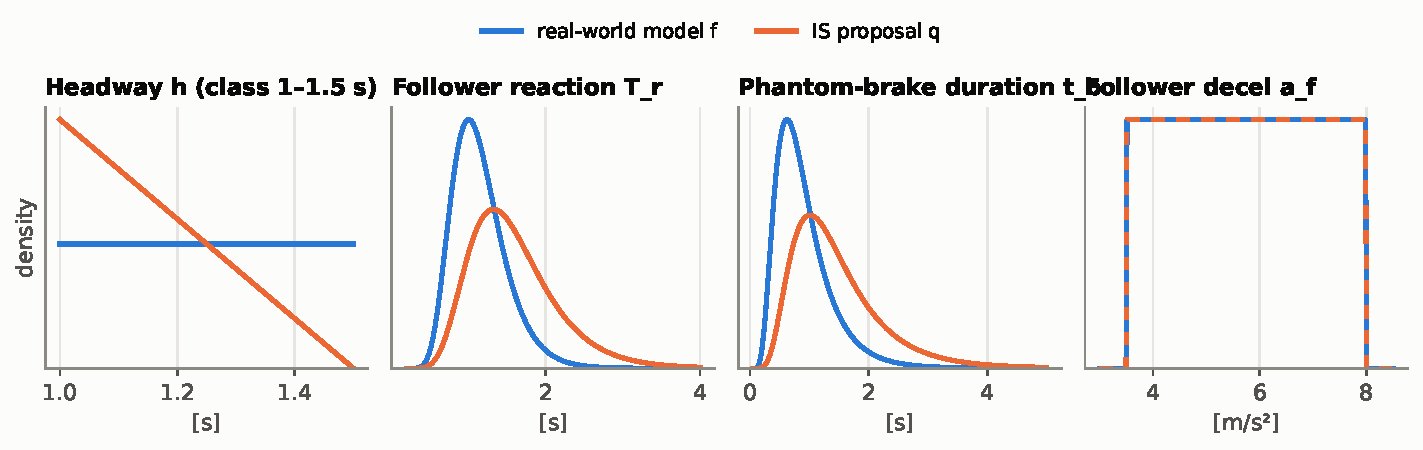
\includegraphics[width=\linewidth]{figures/f09_marginals.pdf}
\caption{Marginals of the real-world model $f$ and the importance-sampling proposal $q$ used in Sec.~\ref{sec:example}\synthetic.}
\end{figure}
\begin{figure}[H]\centering
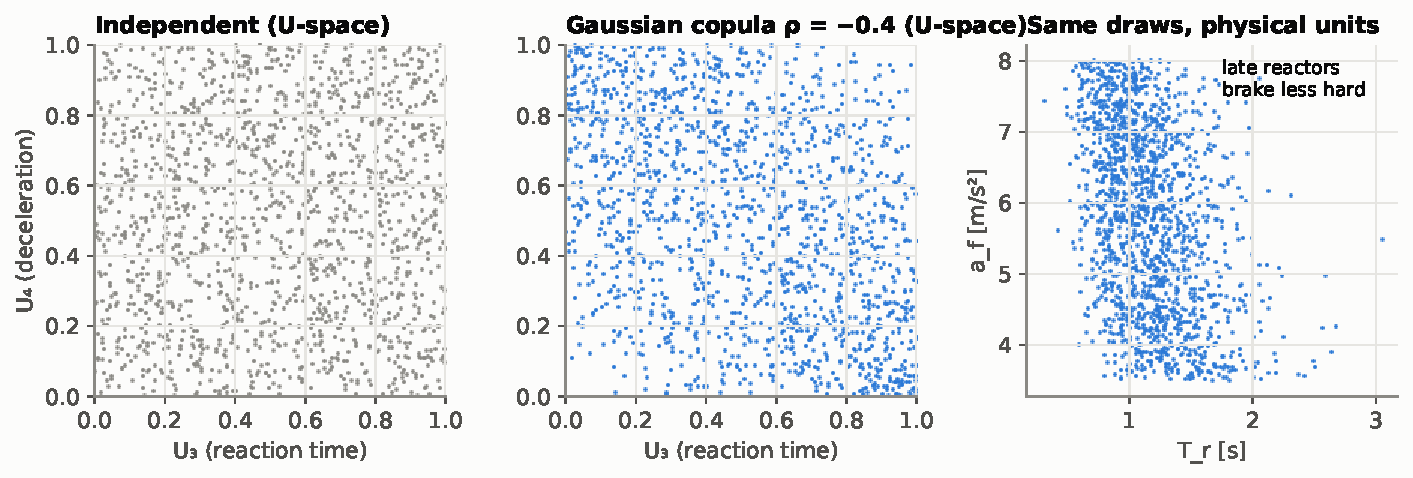
\includegraphics[width=\linewidth]{figures/f10_copula_scatter.pdf}
\caption{Independent uniforms, the Gaussian copula with $\rho=-0.4$, and the same draws in physical units\synthetic.}
\end{figure}

\subsection{Fitting}
Transform each parameter to pseudo-observations $u=\mathrm{rank}/(n+1)$ and normal scores $z=\Phi^{-1}(u)$, and estimate $R$ as their correlation matrix. Pairwise, Kendall's $\tau$ \cite[Ch.~5]{nelsen2006} converts to $\rho=\sin(\pi\tau/2)$ for elliptical copulas \cite[location not verified]{lindskog2003}. $R$ must be positive definite; pairwise estimates may need projection to the nearest correlation matrix.

\subsection{Limitation: no tail dependence}
For $\rho<1$ the Gaussian copula has zero upper tail dependence, whereas the $t$-copula with $\nu$ degrees of freedom has $\lambda_U=2\,t_{\nu+1}\!\big(-\sqrt{(\nu+1)(1-\rho)/(1+\rho)}\big)>0$ \cite[location not verified]{embrechts2003}. Joint extremes, such as a late reaction combined with weak braking, are therefore under-represented if real data show tail dependence (Fig.~\ref{fig:tail}).
\begin{figure}[H]\centering
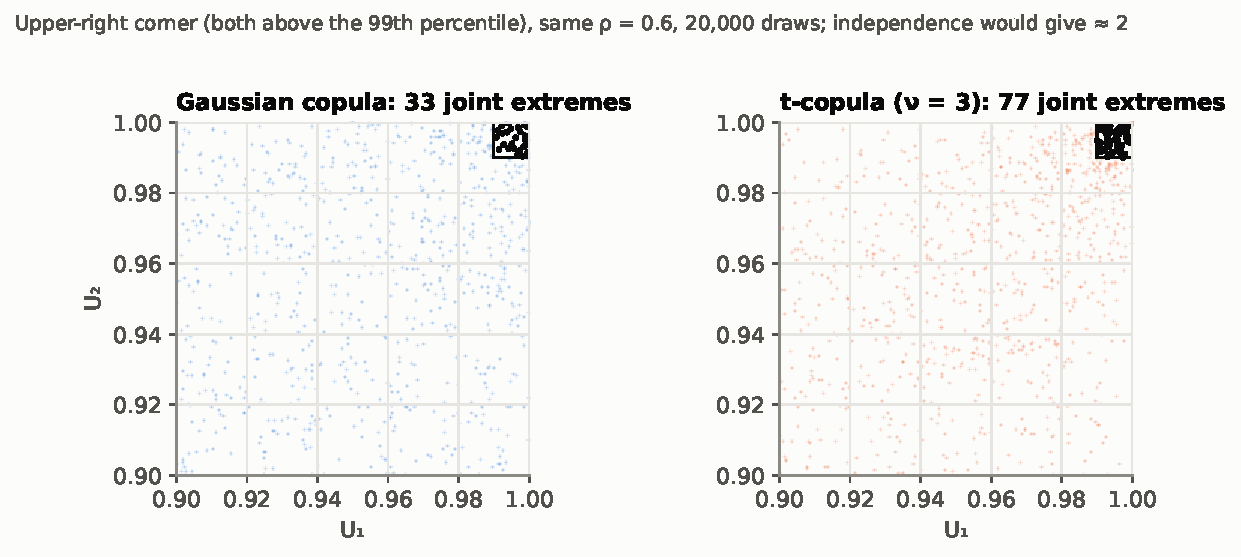
\includegraphics[width=0.9\linewidth]{figures/f11_tail.pdf}
\caption{Same correlation, different joint extremes\synthetic: 33 (Gaussian) versus 77 ($t$, $\nu=3$) draws in the top-1\% corner out of 20{,}000; independence would give about 2 \own{computed}.}
\label{fig:tail}
\end{figure}

%=====================================================================
\section{Worked example: unintended braking with 1{,}000 concrete scenarios}\label{sec:example}
\subsection{Set-up}
\textbf{Everything in this section is synthetic\synthetic.} The set-up follows the structure of the standard's own AEB example, in which unintended braking for longer than 340~ms with a closely following vehicle can lead to a rear-end collision, and a Monte Carlo simulation over trailing distance and reaction time estimates the collision probability \cite[C.2.2.3, Figures~C.1--C.2, pp.~129--130]{iso21448}. The standard finds the collision probability ``higher at lower speeds because of the short trailing distance'' \cite[C.2.2.3, Figure~C.3, pp.~130--131]{iso21448}, as does this example (Fig.~\ref{fig:collinj}). Validation target: MAIS2+ injuries from rear-end collisions caused by unintended (phantom) braking $\le A_H=10^{-7}$/h, with 10\% reserved for unknown triggers, leaving a budget of $9\times10^{-8}$/h. The ODD is partitioned into 100 logical scenarios: 5 trigger contexts $\times$ 4 ego speed bands $\times$ 5 follower-headway classes. The hazardous-behaviour rate $\lambda$ depends on trigger and speed only, so 20 evidence cells serve 100 scenarios. Per logical scenario, 2{,}000 plain runs from $f$ and 10 importance-sampled runs from $q$ are simulated with a one-dimensional kinematic model ($\Delta t=0.01$~s); ego speed, follower headway, reaction time and deceleration are coupled by a Gaussian copula with $\rho(v,h)=0.25$, $\rho(h,T_r)=-0.30$, $\rho(T_r,a_f)=-0.40$. The illustrative injury curve is $P(\text{MAIS2+}\mid\Delta v)=1/(1+e^{-(\Delta v-45)/7})$, $\Delta v$ in km/h \own{App.~\ref{app:code}}.

\begin{figure}[H]\centering
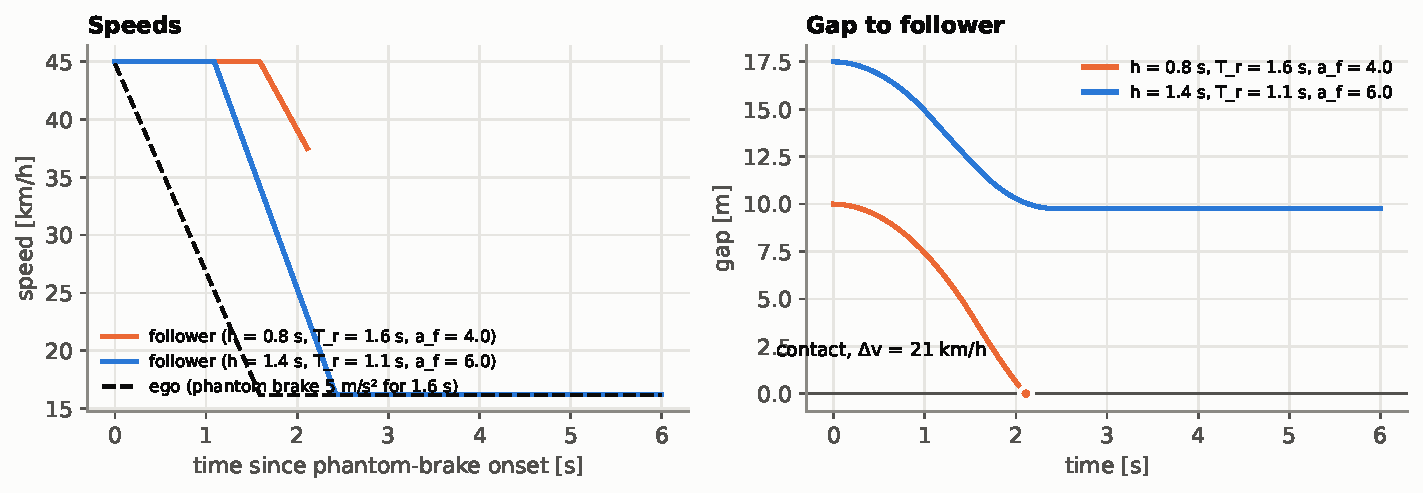
\includegraphics[width=\linewidth]{figures/f13_trajectories.pdf}
\caption{Two concrete scenarios with the same phantom brake\synthetic: contact with a short headway and a late, weak reaction; no contact otherwise.}
\end{figure}

\subsection{Checks of the importance sampling}
On 200{,}000 proposal draws the mean weight is 0.996, and the IS estimate (0.0161) matches 100{,}000 plain runs (0.0157). Over the 1{,}000 concrete scenarios the mean weight is 0.98, weights range from $5\times10^{-4}$ to 67, 117 runs end in a collision, and the median ESS per logical scenario is 4.3 of 10 \own{Fig.~\ref{fig:w}}.
\begin{figure}[H]\centering
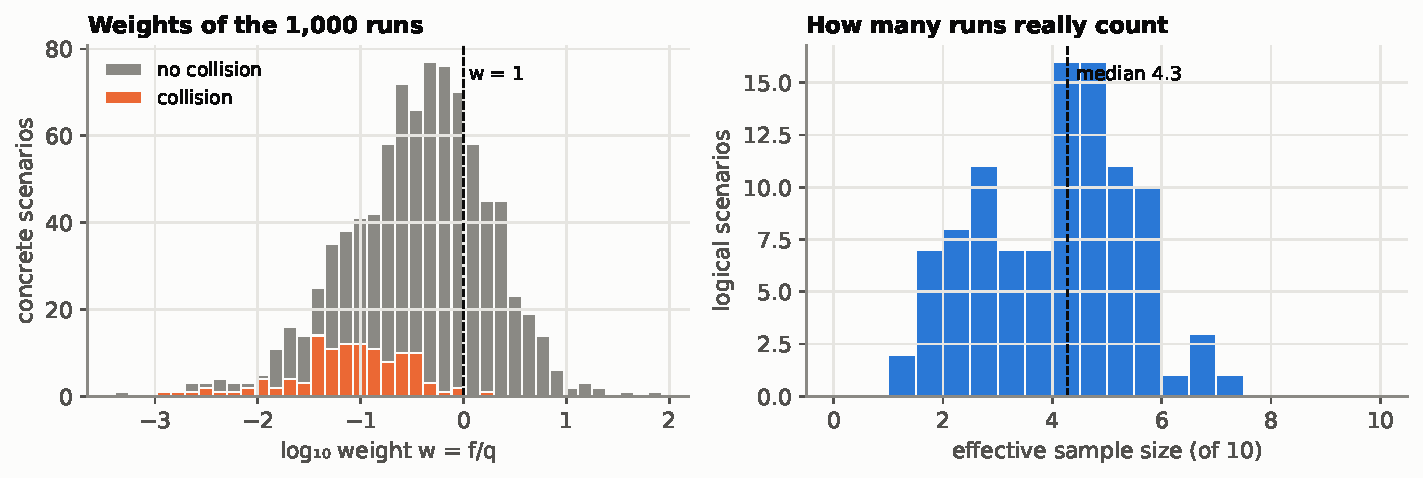
\includegraphics[width=\linewidth]{figures/f14_weights.pdf}
\caption{Weights of the 1{,}000 runs and effective sample size per logical scenario\synthetic.}
\label{fig:w}
\end{figure}
\begin{figure}[H]\centering
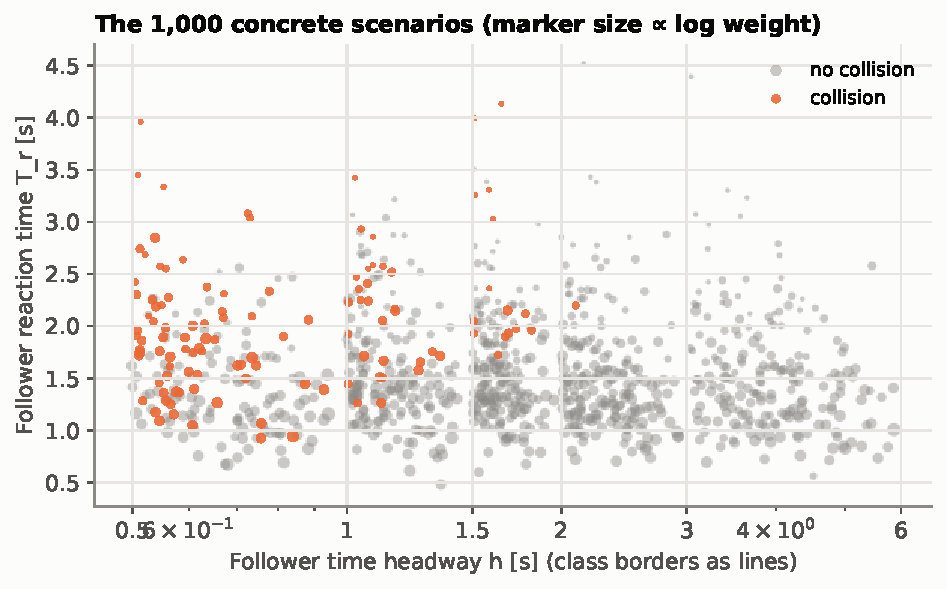
\includegraphics[width=0.86\linewidth]{figures/f15_concrete_scatter.pdf}
\caption{All 1{,}000 concrete scenarios\synthetic; collisions concentrate at short headway and late reaction.}
\end{figure}

\subsection{Results}
\begin{figure}[H]\centering
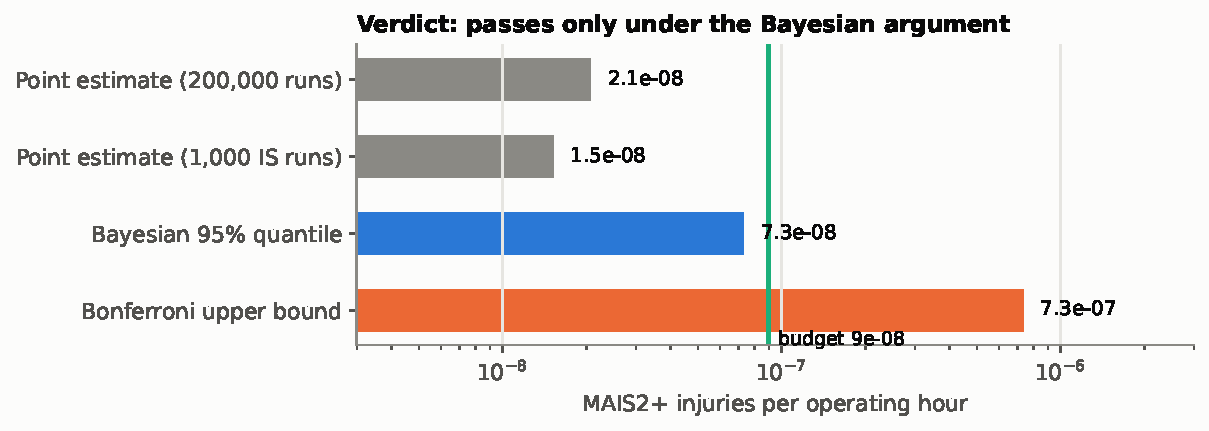
\includegraphics[width=0.9\linewidth]{figures/f16_verdict.pdf}
\caption{Verdict\synthetic: point estimates $2.1\times10^{-8}$ (200{,}000 runs) and $1.5\times10^{-8}$/h (1{,}000 IS runs), Bayesian 95\% quantile $7.3\times10^{-8}$/h (passes), Bonferroni bound over 120 estimates $7.3\times10^{-7}$/h (fails) \own{computed}.}
\end{figure}
\begin{figure}[H]\centering
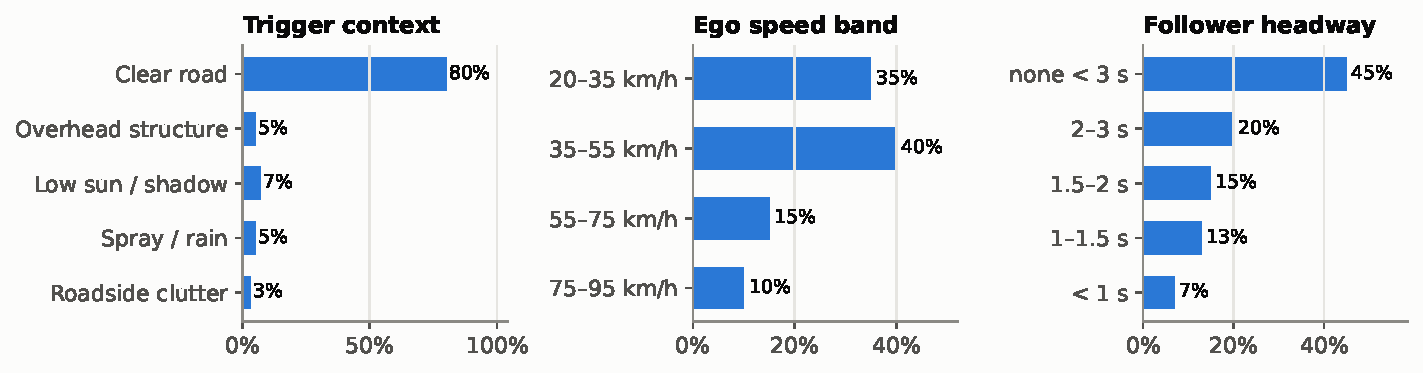
\includegraphics[width=\linewidth]{figures/f17_exposure.pdf}
\caption{Exposure shares per factor\synthetic; scenario share = product (independence assumed).}
\end{figure}
\begin{figure}[H]\centering
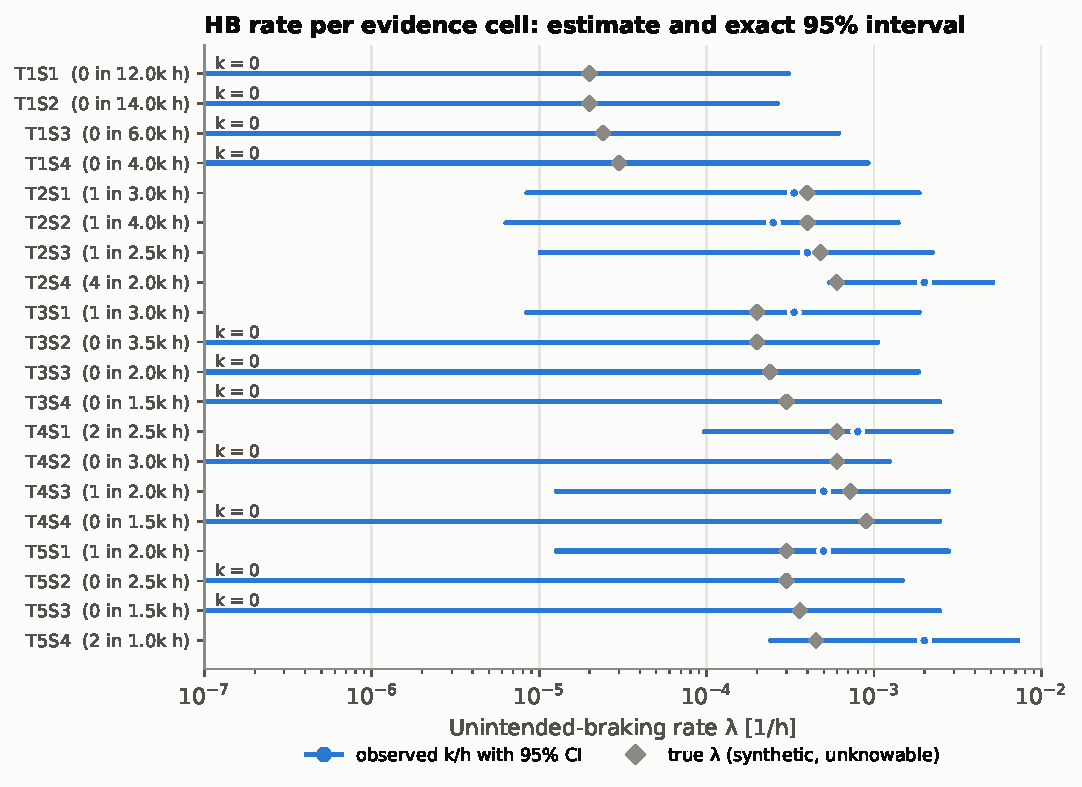
\includegraphics[width=0.86\linewidth]{figures/f18_hb.pdf}
\caption{Hazardous-behaviour rate per evidence cell\synthetic: observed $k/h$ with exact 95\% interval, and the synthetic true rate.}
\end{figure}
\begin{figure}[H]\centering
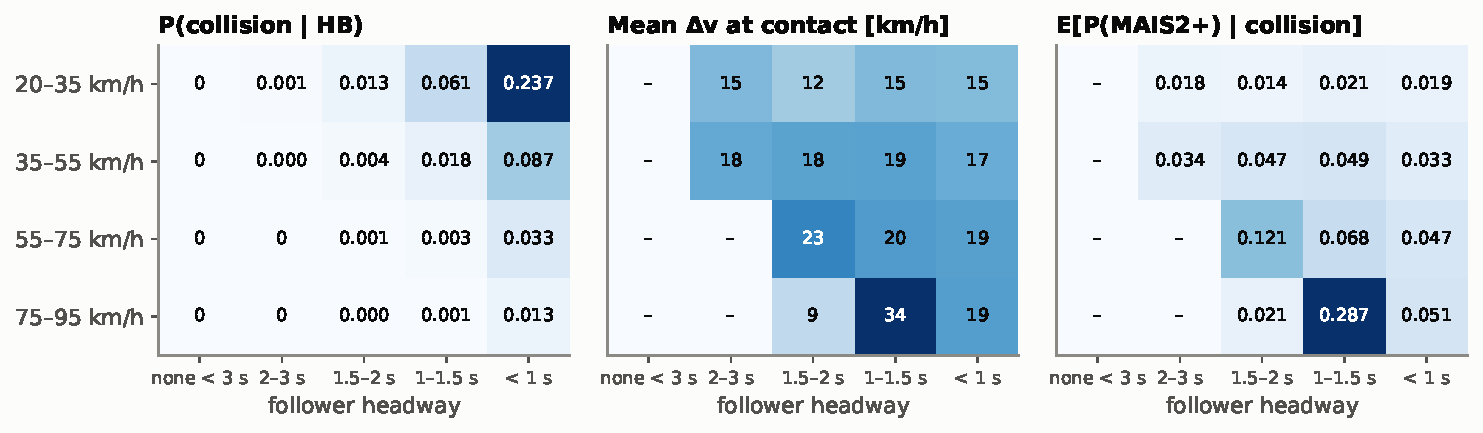
\includegraphics[width=\linewidth]{figures/f19_coll_inj.pdf}
\caption{Collision probability, mean $\Delta v$ and injury probability by speed band and headway\synthetic.}\label{fig:collinj}
\end{figure}
\begin{figure}[H]\centering
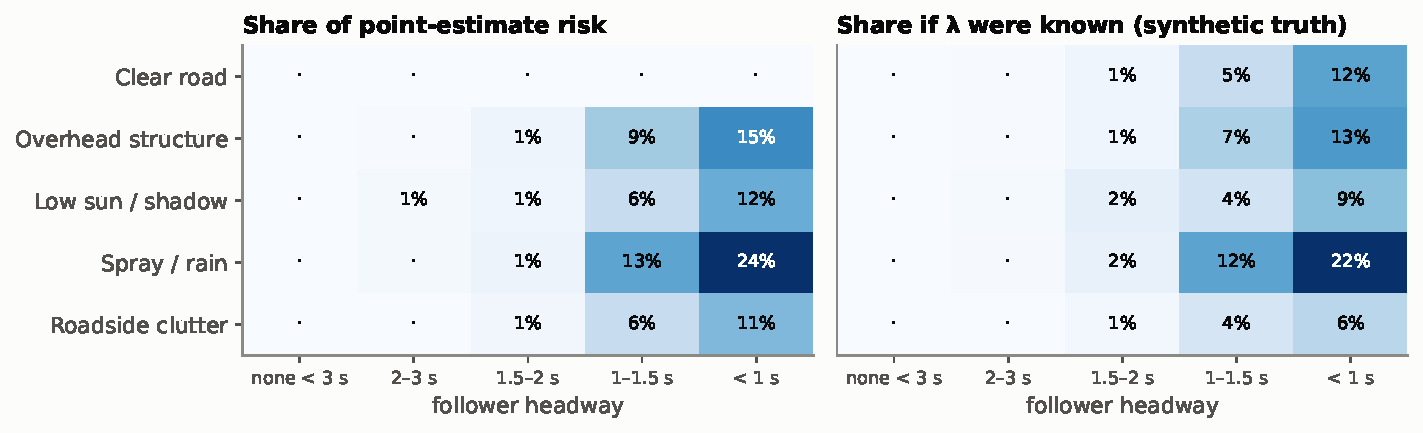
\includegraphics[width=\linewidth]{figures/f20_risk_share.pdf}
\caption{Where the risk sits\synthetic: attribution from observed counts (left) against attribution with the true rates (right). With 0--4 events per cell, point-estimate attribution is largely Poisson noise.}
\end{figure}
\begin{figure}[H]\centering
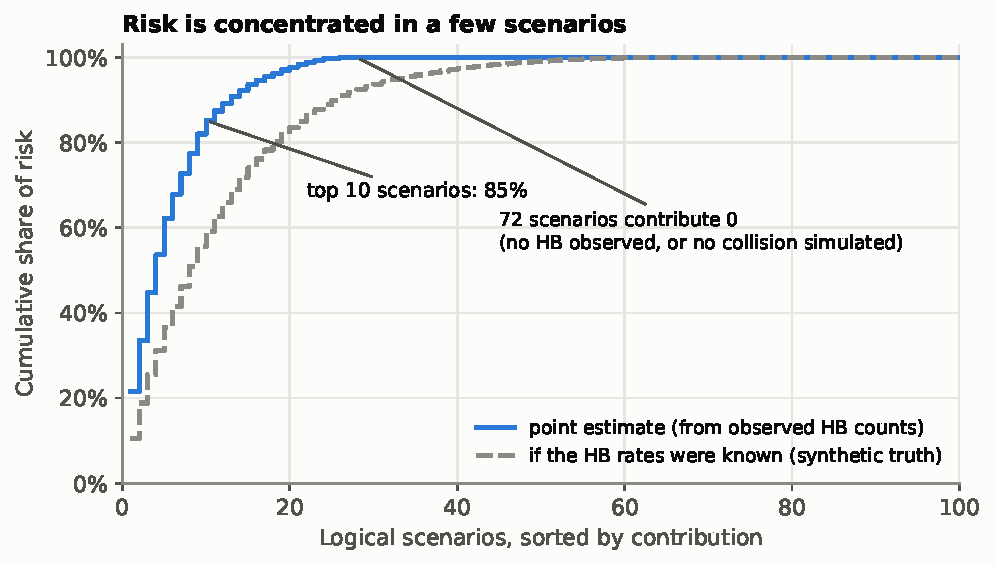
\includegraphics[width=0.86\linewidth]{figures/f03_pareto.pdf}
\caption{Cumulative share of the point estimate over the 100 logical scenarios\synthetic; the top 10 carry 85\%.}
\end{figure}
\begin{figure}[H]\centering
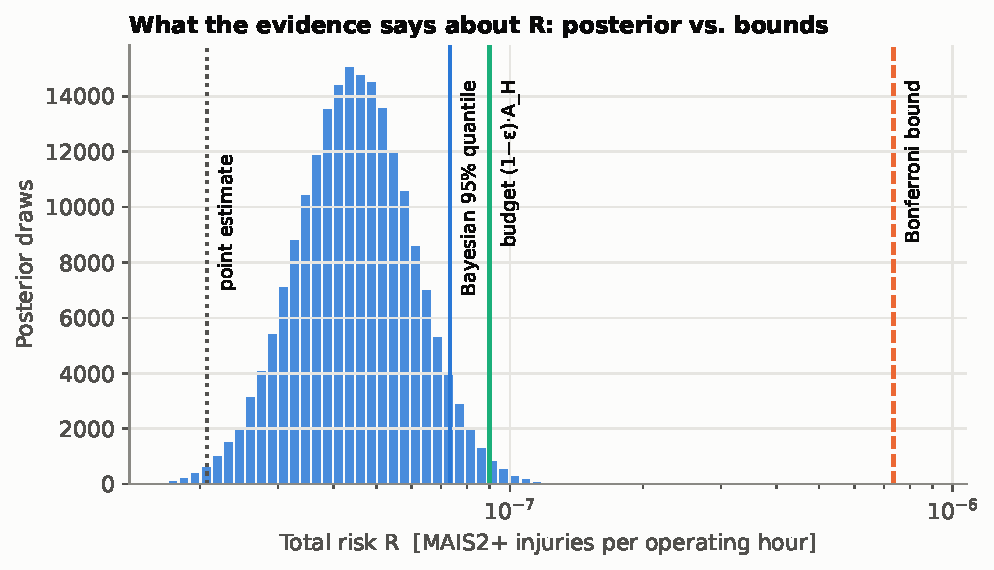
\includegraphics[width=0.86\linewidth]{figures/f04_posterior.pdf}
\caption{Posterior of total risk with Jeffreys priors\synthetic, against point estimate, budget and Bonferroni bound. Jeffreys and flat priors as discussed in \cite[Sec.~V, RA ``Bayesian Statistics'']{betschinske2025}.}
\end{figure}
\begin{figure}[H]\centering
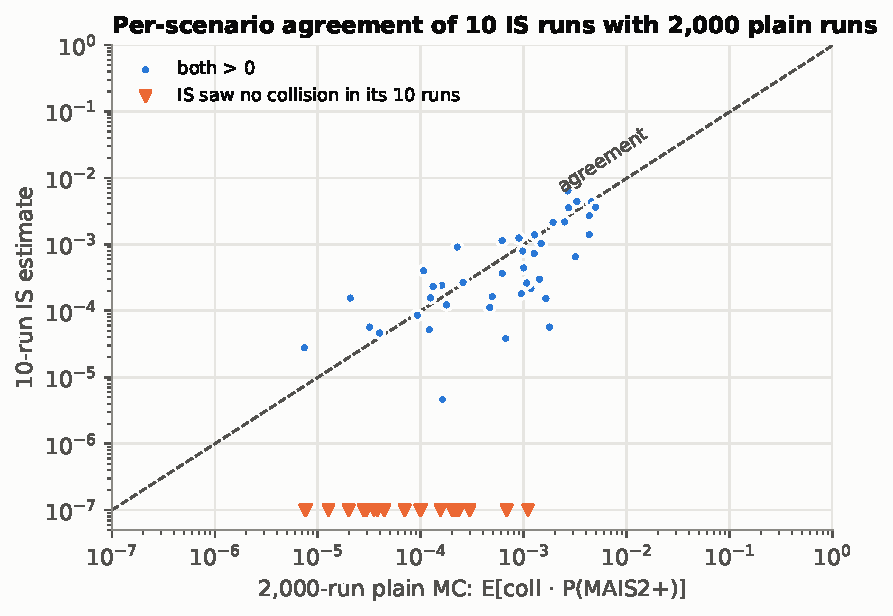
\includegraphics[width=0.8\linewidth]{figures/f21_is_vs_mc.pdf}
\caption{Per-scenario agreement of 10 IS runs with 2{,}000 plain runs\synthetic. 22 scenarios saw no collision in their 10 IS runs although plain Monte Carlo did.}
\end{figure}
\begin{figure}[H]\centering
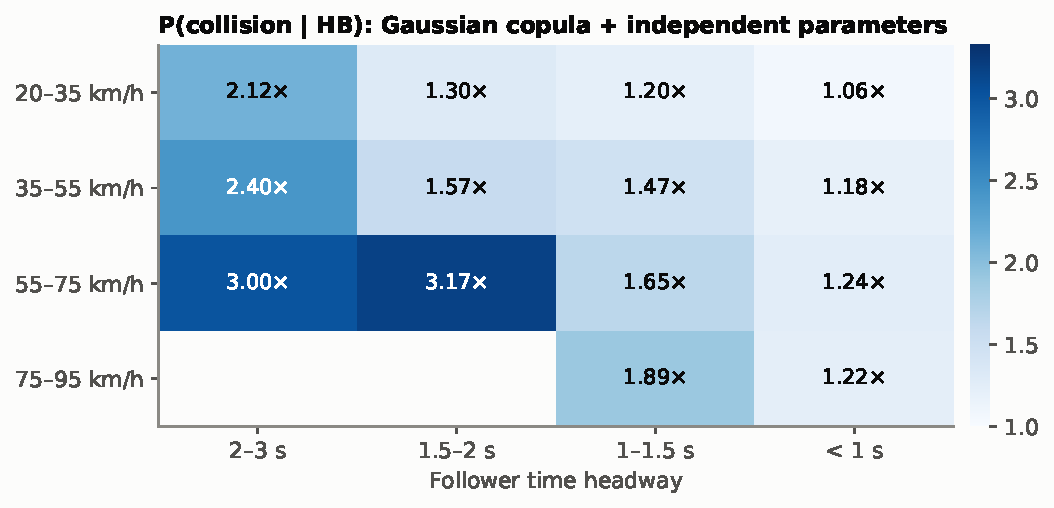
\includegraphics[width=0.86\linewidth]{figures/f12_copula_heat.pdf}
\caption{Ratio of $P(\text{collision}\mid\mathrm{HB})$ with the Gaussian copula to the same model with independent parameters, 20{,}000 runs per cell\synthetic: 1.06 to 3.2.}
\end{figure}

\subsection{Evidence needed}
Minimising total test hours $\sum_j \lambda_{k,j} G_j/B_j$ subject to $\sum_j B_j=B$, with $G_j$ the harm weight of cell $j$ and $\lambda_{k,j}=\tfrac12\chi^2_{2(k_j+1)}(C_b)$ its Poisson factor, gives
\begin{equation}
B_j = B\,\frac{\sqrt{\lambda_{k,j}G_j}}{\sum_i\sqrt{\lambda_{k,i}G_i}},\qquad T_{\text{total}}=\frac{\big(\sum_j\sqrt{\lambda_{k,j}G_j}\big)^2}{B}
\label{eq:alloc}
\end{equation}
\own{Lagrange multiplier}. For the Bonferroni claim, 564{,}100~h are required against 73{,}500~h available (Fig.~\ref{fig:targets}). (An earlier version used $B_j\propto\sqrt{G_j}$, which is optimal only if all cells have the same $k_j$; Sec.~\ref{sec:audit}.)
\begin{figure}[H]\centering
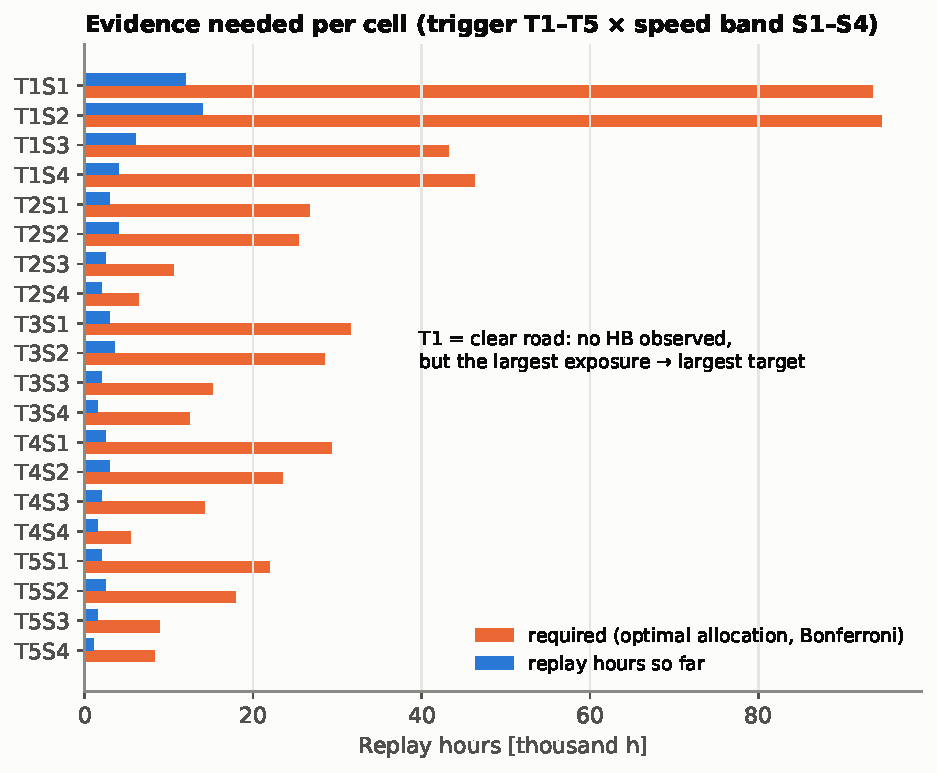
\includegraphics[width=0.86\linewidth]{figures/f05_evidence_targets.pdf}
\caption{Replay hours per evidence cell, available versus required under the square-root allocation\synthetic.}
\label{fig:targets}
\end{figure}

%=====================================================================
\section{Field data, statistics and safety performance indicators}\label{sec:field}
\subsection{Data to collect}
\begin{table}[H]\centering\small
\caption{Field data organised by the term of Eq.~\eqref{eq:risk} it feeds.}
\begin{tabular}{L{2.8cm}L{7.4cm}L{4.2cm}}
\toprule
Feeds & Data & How\\\midrule
exposure & hours and km with ODD tags per time step, including periods without any scenario & continuous signals plus map and weather lookup\\
scenario distributions & every occurrence with its parameters & scenario tagger \cite[Sec.~III]{guo2023}\\
HB rate & every brake request with its cause, plus suppressed near-HBs & event-triggered raw-data buffer\\
perception error model & misses and false positives against labelled ground truth, by class, range, occlusion, weather & labelled samples\\
outcomes & collisions with $\Delta v$, near-miss surrogates (min TTC, PET) & rear sensors, incident process\\
responses & minimal-risk manoeuvres, remote assistance, monitor flags \cite[Sec.~4]{schaller2026} & system logs\\
provenance & software hash, configuration, map version, calibration & attached to every hour\\
\bottomrule
\end{tabular}
\end{table}
Clause~13 lists as topics for observation incidents that caused or could have caused harm or exceeded defined values, the body of knowledge, and context evolution \cite[13.3~a)--c), pp.~56--57]{iso21448}. For higher levels of automation it names on-board monitoring that detects functional insufficiencies before accidents occur, e.g.\ capturing violations of a minimum distance, scenarios close to triggering a system reaction, unexpected take-overs and scenarios leading to a minimal risk condition, and data storage such as DSSAD/EDR \cite[13.3, Note~1 and Examples~1--2, p.~56]{iso21448}. These are leading SPIs in the sense of Sec.~\ref{sec:spi}.

\subsection{Statistics}
Rates are bounded with Eq.~\eqref{eq:chi2} per stratum and software version (Fig.~\ref{fig:rate}); binomial proportions with Clopper--Pearson bounds \cite[location not verified]{clopper1934}. Near misses can be extrapolated to crash frequencies with extreme value analysis: a generalised Pareto distribution is fitted to exceedances over a threshold \cite[Ch.~4]{coles2001}; Betschinske et al.\ review its use for validation and its open issues \cite[Sec.~V, RA ``Extreme Value Analysis'', Table~IX]{betschinske2025}.
\begin{figure}[H]\centering
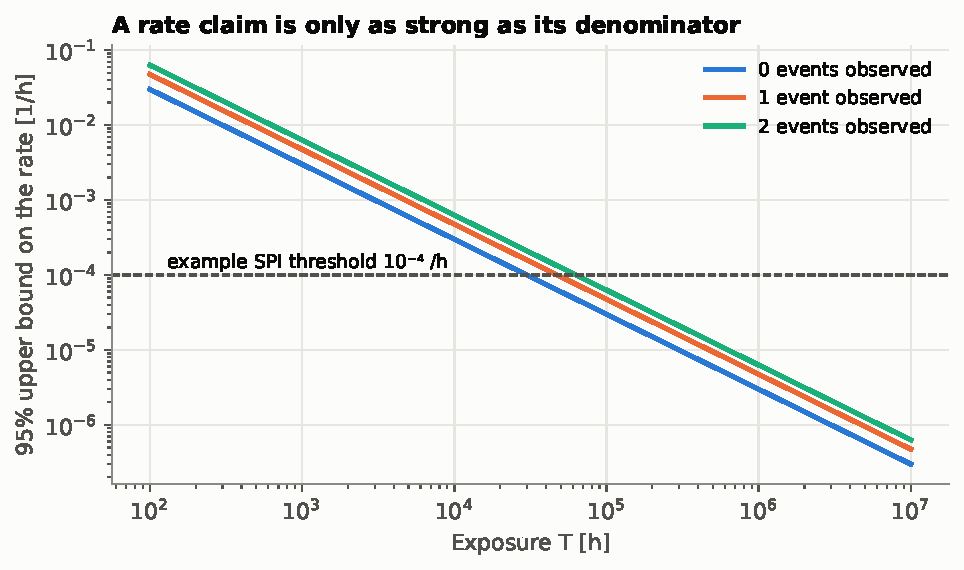
\includegraphics[width=0.82\linewidth]{figures/f06_rate_bound.pdf}
\caption{95\% upper bound on a rate against exposure for 0, 1, 2 observed events \own{Eq.~\eqref{eq:chi2}}.}
\label{fig:rate}
\end{figure}
\begin{figure}[H]\centering
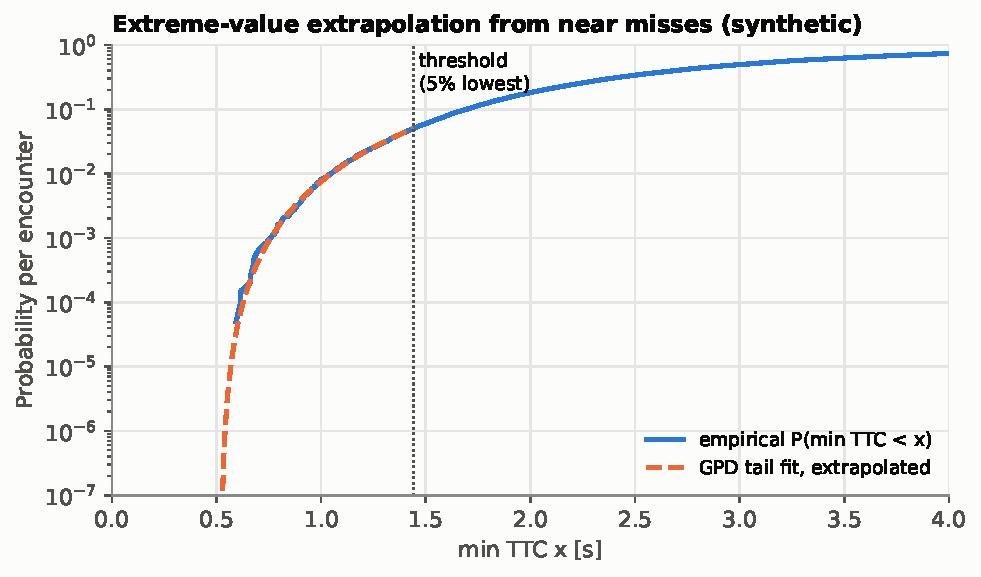
\includegraphics[width=0.82\linewidth]{figures/f08_evt.pdf}
\caption{Extreme-value extrapolation of synthetic minimum-TTC data\synthetic: the lowest 5\% are fitted with a generalised Pareto tail and extrapolated.}
\end{figure}

\subsection{Safety performance indicators}\label{sec:spi}
UL~4600 defines: ``An SPI is a metric supported by evidence that uses a threshold comparison to condition a claim in a safety case'' (UL~4600, as cited in \cite[Sec.~2, ``UL4600'']{ratiu2024}), and states that ``relying solely on lagging indicators is not acceptable'' (UL~4600 note 16.2.2.6.2, as cited in \cite[Sec.~2]{ratiu2024}). Lagging indicators detect shortcomings from past events; leading indicators identify potential issues before losses, e.g.\ unexpected fail-safe activations \cite[Sec.~2]{ratiu2024}. Koopman contrasts KPIs (``how well do we drive'') with SPIs (``how often are we potentially unsafe'') \cite[slide~12]{koopman2022}, lists lagging SPIs \cite[slide~6]{koopman2022} and leading SPIs \cite[slide~7]{koopman2022}, and gives examples such as a false negative for more than $k$ consecutive frames and violations of a safe clearance limit \cite[slide~10]{koopman2022}. An SPI violation means its claim is violated, but a claim can be violated without its SPI firing \cite[Sec.~2; Sec.~3.1]{ratiu2024}. Responses range from updating the safety case and SPIs, through restricting operation (reduced speed, geofences) and updating the system, to grounding the fleet \cite[Sec.~3.3]{ratiu2024}.

\begin{table}[H]\centering\small
\caption{Example SPI register for unintended braking \own{Sec.~\ref{sec:example}}.}
\begin{tabular}{L{1.7cm}L{5.2cm}L{3.8cm}L{3.6cm}}
\toprule
Type & SPI & Claim conditioned & Threshold\\\midrule
lagging & rear-end collisions with ego struck, per h, by severity & overall target & $A_H$\\
leading & unexplained brake requests per 1{,}000 h per trigger context & HB rate per context & $\lambda$ target, Fig.~\ref{fig:targets}\\
leading & suppressed false-positive brake detections & margin before HB & trend alarm\\
leading & rear TTC $<1.5$~s within 3~s after ego braking & $P(\text{coll}\mid\mathrm{HB})$ & simulation prediction\\
safety case & share of time with follower $<1$~s & exposure assumption & $\chi^2$ test\\
safety case & Kendall's $\tau$(headway, reaction) & copula assumption & CI contains assumed $\rho$\\
safety case & rate of unclassifiable scenarios & reserve $\varepsilon$ & Eq.~\eqref{eq:unk}\\
\bottomrule
\end{tabular}
\end{table}

The time an SPI needs to detect a doubling of its rate depends only on the expected count: for a one-sided exact Poisson test at $\alpha=0.05$ and power 0.8 it takes $\mu^*\approx 9.1$ expected events, so $T=\mu^*/\lambda$ \own{computed}. Lagging SPIs near the acceptance criterion would take decades to centuries for a 50-vehicle fleet (Fig.~\ref{fig:detect}).
\begin{figure}[H]\centering
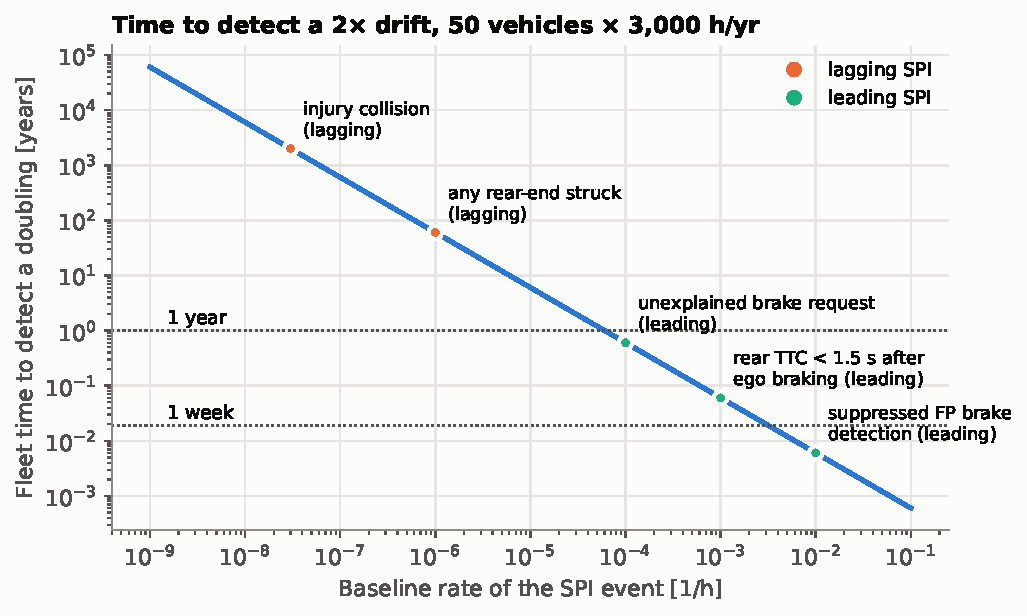
\includegraphics[width=0.86\linewidth]{figures/f07_detect.pdf}
\caption{Fleet time to detect a 2$\times$ drift for 50 vehicles $\times$ 3{,}000~h/yr \own{computed}.}
\label{fig:detect}
\end{figure}

%=====================================================================
\section{L4 validation, the scenario database and completeness}\label{sec:l4}
\subsection{Vehicle-level V\&V strategy}
Note that ISO~21448 reserves ``vehicle-level SOTIF strategy'' for a set of vehicle-level requirements (Sec.~\ref{sec:framework}) \cite[3.34, p.~10]{iso21448}; the strategy below is the V\&V strategy of Clause~9.
\begin{table}[H]\centering\small
\caption{Pillars of the vehicle-level V\&V strategy (ISO~21448 Clause~9) and the term they feed.}
\begin{tabular}{L{5.4cm}L{2.4cm}L{6.4cm}}
\toprule
Pillar & SOTIF & Feeds\\\midrule
ODD spec, HARA, triggering-condition analysis & Cl.~5--7 & $A_s$, HB/HE list, scenario taxonomy\\
component V\&V: perception KPIs per ODD stratum, planner checks & Cl.~10 & perception error models\\
scenario-based simulation from the database & Cl.~10 & $p_\ell$, coverage \cite[Sec.~6.2, pp.~16--17]{schaller2026}\\
log replay, XiL, proving ground & Cl.~10 & $\lambda$ per context; sim-to-real bounds\\
public-road exploration and FOT & Cl.~11 & $\nu$, $f$, $R_{\text{unknown}}$ \cite[Sec.~6.3, p.~17]{schaller2026}\\
shadow mode, operation & Cl.~13 & SPIs \cite[Sec.~7, p.~18]{schaller2026}\\
release argument & Cl.~12 & Eq.~\eqref{eq:claim} per harm\\
\bottomrule
\end{tabular}
\end{table}
ISO~21448 expects validation to combine physical (test track, real-world) and simulation testing, with the quantitative target often allocated between them \cite[C.1, p.~125]{iso21448}, and the V\&V strategy to address the ODD boundaries and outside of the ODD as part of the coverage argument \cite[9.2 and Note, p.~43]{iso21448}. The structure matches the NATM pillars of virtual, track and real-world testing, audit and in-service monitoring \cite[web article]{siemensnatm}. Schaller et al.\ show how a runtime monitor ensemble contributes evidence to Clauses~6, 9--11 and~13 without by itself establishing SOTIF compliance \cite[Sec.~1.2, p.~3; Secs.~5--7, pp.~14--18]{schaller2026}, and propose that the standard make explicit that residual risk can be quantified from a statistical argument over traffic situations sourced from monitoring data \cite[Sec.~8.2, p.~19]{schaller2026}.

\subsection{What the scenario database contributes}
\begin{enumerate}
\item It makes ``known'' explicit: the taxonomy is the boundary between known and unknown scenarios.
\item It holds the weights $\nu_\ell$ and $f_\ell(\theta)$, derived from recordings.
\item It generates tests and keeps traceability from triggering condition to hazardous behaviour, hazardous event, requirement and test.
\item It shows coverage per scenario $\times$ triggering condition $\times$ software version.
\item It stores every run with $\theta$, $q(\theta)$, software hash and outcome, so risk can be recomputed after changes.
\item It moves unknown to known: discovered types become categories.
\end{enumerate}
\begin{lstlisting}
Recording(id, vehicle, sw_hash, map_ver, calib_state, route, hours, raw_uri)
ExposureSlice(recording_id, t0, t1, odd_tags...)        -- denominators
ScenarioCategory(id, version, tag_rule, param_schema, partition_key)
Occurrence(id, recording_id, t0, t1, category_id, theta..., odd_tags, min_ttc, hb_flag)
HazardLink(category_id, hb_id, he_id, triggering_condition_id)
TestRun(id, category_id, theta..., q_density, platform, sw_hash, outcome, dv)
\end{lstlisting}

\subsection{From recordings to the database}
Raw logs are turned into a reference world model by offline perception and labels, enriched with map, weather and ODD tags for every time step, tagged with actor activities and interactions, and converted into scenario occurrences with parameters read at defined anchor events. This is the tag-based pipeline of Guo et al.: preprocessing \cite[Sec.~III-A]{guo2023}, tagging of actor activities \cite[Sec.~III-B.1]{guo2023} and interactions \cite[Secs.~III-B.2, III-B.3]{guo2023}, and categorisation by tag combinations \cite[Sec.~III-C]{guo2023}, applied to the Waymo Open Motion Dataset and CARLA data \cite[Sec.~IV]{guo2023}. Four rules matter: extract with a reference world model, not the stack under test; tag every driven second; attach provenance and a pointer to the raw log window; version the taxonomy and re-tag historical data when it changes.

\subsection{Identifying scenarios automatically}
\textbf{Known types.} Guo et al.\ report no incorrect extraction among 116 randomly examined of 215{,}090 extracted WOMD scenarios, but no precision or recall of individual tags \cite[Sec.~IV]{guo2023}. A tagger is a classifier, and its errors bias exposure. With measured precision and recall, $\hat\nu_\ell=n_{\text{detected}}\cdot\text{precision}/(\text{recall}\cdot T)$ \own{Fig.~\ref{fig:tagger}}.
\begin{figure}[H]\centering
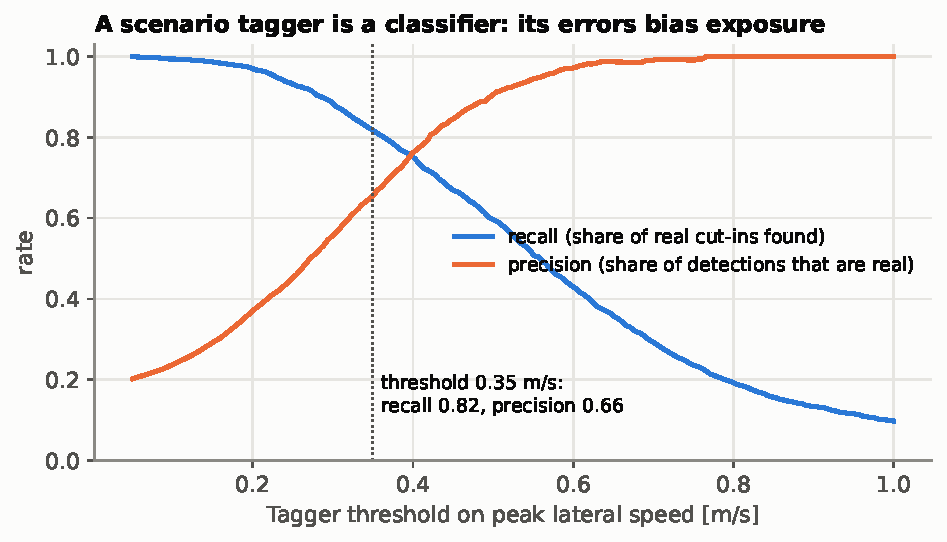
\includegraphics[width=0.82\linewidth]{figures/f24_tagger.pdf}
\caption{Synthetic cut-in tagger\synthetic: at 0.35~m/s it finds 82\% of real cut-ins, and 66\% of its detections are real \own{computed}.}
\label{fig:tagger}
\end{figure}
\textbf{New types (Clause~11).} (1) A queue of unexplained critical events (low TTC, hard braking, HB flags, monitor flags, disengagements) that match no category, for human review; Schaller et al.\ propose monitors that flag novel input/output behaviour and unfamiliar activation patterns as candidates for hazard identification \cite[Sec.~5.1, pp.~14--15]{schaller2026}. (2) Unsupervised clustering of time-window embeddings with outlier flags \cite[Abstract]{unsupervised2022}. (3) ODD novelty: conditions outside the specification or rare tag combinations.

\subsection{ODD tags: coverage and granularity}
ISO~34503 specifies the ODD taxonomy \cite[location not verified]{iso34503} and ISO~34504 a tag-based scenario categorisation; ISO~34504 ``provides examples rather than instructions on its application and tags'' and does not fix values such as the speed difference in ``moving faster or slower'' \cite[web article]{tno2024}. Both are a shared vocabulary, not a sufficient resolution. Tags missing for a given function (overhead structures, road spray or low sun for phantom braking) are derived from the triggering-condition analysis and from structured environment models: Reich's SEM use guide phrases with an environment ontology to identify the environment factors that influence hazardous situations and their risks \cite[Sec.~1.3, p.~4]{reich2026}, giving a hazard-specific environment model with explicit coverage checks \cite[Sec.~1.4, contribution~1.1, p.~6; Sec.~4.1, p.~49]{reich2026}.

\textbf{Granularity criterion.} A class may lump values together if a shift of the distribution inside the class cannot move the risk materially:
\begin{equation}
|\Delta R_c|=\nu_c\Big|\int_c p(\theta)\big(f^{\text{dep}}_c-f^{\text{test}}_c\big)d\theta\Big|\le \nu_c\,(p^{\max}_c-p^{\min}_c)\,\mathrm{TV}\big(f^{\text{dep}}_c,f^{\text{test}}_c\big)
\end{equation}
where $\mathrm{TV}(f,g)=\sup_A|P_f(A)-P_g(A)|=\tfrac12\int|f-g|$ is the total-variation distance (the bound uses $\int(f-g)=0$ and fails by a factor 2 if TV is read as the $L^1$ distance) \own{derived}. Classes are refined until the sum over classes fits a reserved share $\delta$ of the budget. In the example, $P(\text{collision}\mid\mathrm{HB})$ falls from 0.137 to 0.030 inside the shortest headway class, while the 2--3~s class is flat (Fig.~\ref{fig:gran}).
\begin{figure}[H]\centering
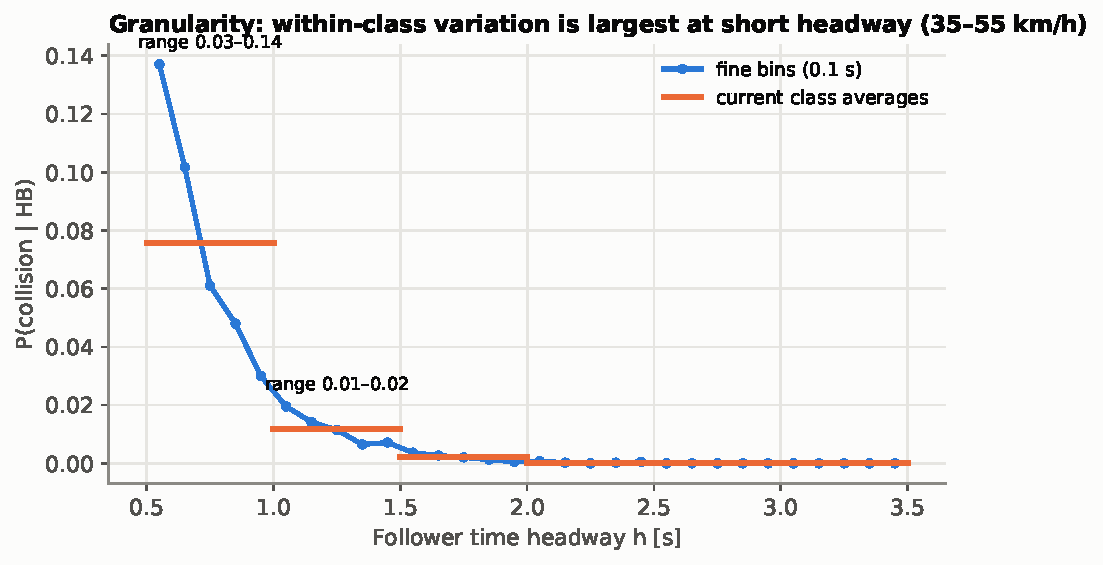
\includegraphics[width=0.86\linewidth]{figures/f23_granularity.pdf}
\caption{$P(\text{collision}\mid\mathrm{HB})$ on a 0.1~s grid against current headway classes\synthetic.}
\label{fig:gran}
\end{figure}

\textbf{Combinatorial coverage.} ISO~21448 lists random combinations of known parameters and of known scenarios among the tests addressing area~3 \cite[C.1, items~1)--2), p.~125]{iso21448}. De Gelder et al.\ define tag-based coverage
\begin{equation}
\text{Coverage}_{\text{tag}}(n)=\frac{1}{n|L||C|}\sum_L\sum_C\min\big(n,N(L,C)\big)
\end{equation}
\cite[Sec.~III-A, Eq.~(1)]{degelder2024}, together with time-based, actor-based and actor-over-time coverage \cite[Secs.~III-B--III-D, Eqs.~(2)--(4)]{degelder2024}. On HighD with 10 categories and 18 tags, $\text{Coverage}_{\text{tag}}(10)=1$ \cite[Sec.~IV-B]{degelder2024}, while about 75\% of time instants are covered by at least one scenario \cite[Sec.~IV-C]{degelder2024}. Applied to tag pairs, the metric exposes untested combinations (Fig.~\ref{fig:pairs}).
\begin{figure}[H]\centering
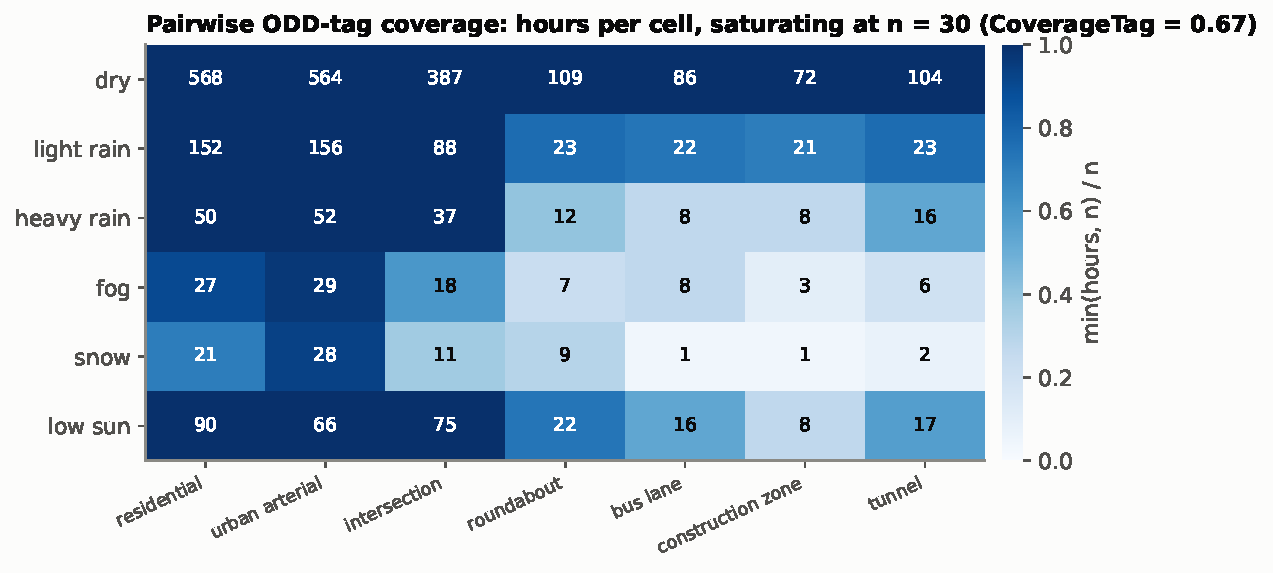
\includegraphics[width=0.9\linewidth]{figures/f25_pair_coverage.pdf}
\caption{Synthetic exposure hours per weather $\times$ road-type pair\synthetic: 26 of 42 pairs have fewer than 30~h; $\text{Coverage}_{\text{tag}}(30)=0.67$ \own{computed}.}
\label{fig:pairs}
\end{figure}

\subsection{Arguing completeness}
Glasmacher et al.\ argue the completeness of a scenario concept in goal structuring notation by testing counter-hypotheses \cite[Sec.~III-C; applied in Sec.~IV-B]{glasmacher2024}. They define completeness as binary and applying to the concept, and coverage as quantifiable and applying to parameter spaces and value assignments \cite[Secs.~III-A, III-B]{glasmacher2024}; evidence is knowledge-based or data-driven \cite[Sec.~III-D, Table~I]{glasmacher2024}. On inD they assign 59{,}253 base scenarios with no unassigned seconds and use saturation curves \cite[Sec.~IV-C, Fig.~5]{glasmacher2024}, noting that ``unforeseen scenarios cannot be identified with argumentation, but with external input'' \cite[Sec.~IV-C]{glasmacher2024} and that completeness claims can expire and need review in a dev-ops process \cite[Sec.~V]{glasmacher2024}. De Gelder et al.\ distinguish Type~I coverage (all relevant aspects of the ODD) from Type~II (all relevant aspects in the driving data) \cite[Sec.~III, Table~III]{degelder2024} and leave completeness metrics to future work \cite[Secs.~V--VI]{degelder2024}. Table~11 of ISO~21448 lists ``scenario exploration in real world'', defined as searching ``for unknown scenarios by covering a diverse set of the real-world scenarios'' \cite[11.3, Table~11, method~O and footnote~e, p.~51]{iso21448}. Hauer et al.\ \cite{hauer2019} estimate the number of scenario types not yet addressed in testing (as summarised in \cite[Sec.~II]{degelder2024}).

ISO~21448 requires ``sufficient coverage of the relevant scenario space'' in the V\&V strategy \cite[9.1~a)~2), p.~42]{iso21448}, notes ``a representative coverage of the possible scenario space'' as one aspect of Clause~11 \cite[11.1, Note, p.~50]{iso21448}, and describes an iterative constrained-random process that converts area~3 into area~2 ``until sufficient coverage of the used functionality space is achieved'' \cite[C.3, Figure~C.4, p.~135]{iso21448}. Five legs of an argument follow:
\begin{enumerate}
\item construction: systematic derivation of the taxonomy, independent review;
\item explained time: the share of driven time assigned to a category (Type~II coverage);
\item saturation: a flattening discovery curve and small missing mass;
\item risk-weighted remainder: bounded by Clause~11 field evidence within the reserve $\varepsilon A_H$;
\item monitoring in operation, because completeness claims expire: new unknown hazardous scenarios can arise with algorithm, ODD, OEDR or driving-policy changes and new vehicle types \cite[11.3, Note~1, p.~52]{iso21448}.
\end{enumerate}
For leg~3, the Good--Turing estimate of the probability that the next occurrence is of an unseen type \cite[location not verified]{good1953} and the Chao1 richness estimator \cite[location not verified]{chao1984} are
\begin{equation}
\hat M_0=\frac{f_1}{N},\qquad \hat S=S_{\text{obs}}+\frac{f_1(f_1-1)}{2(f_2+1)},\qquad R_{\text{unknown}}\lesssim \hat M_0\,\nu_{\text{tot}}\,\bar p_{\text{unk}}
\label{eq:unk}
\end{equation}
with $f_1,f_2$ the numbers of types seen once or twice and $N$ the number of occurrences. $\hat M_0$ is a point estimate. For an upper confidence bound, the missing mass $U_N$ satisfies $P(U_N > E\,U_N+\varepsilon)\le e^{-N\varepsilon^2}$ \cite[Theorem~1]{berend2013}, so $U_N\le E\,U_N+\sqrt{\ln(1/\delta)/N}$ with probability at least $1-\delta$; a rigorous bound also accounts for the deviation of the Good--Turing estimate from $E\,U_N$ \cite[location not verified]{mcallester2000}. In the synthetic example ($N=200{,}000$, $\delta=0.05$) the concentration term $\sqrt{\ln 20/N}=3.9\times10^{-3}$ is larger than $\hat M_0=1.1\times10^{-3}$ itself \own{computed}: saturation data bound the unknown mass only weakly.
\begin{figure}[H]\centering
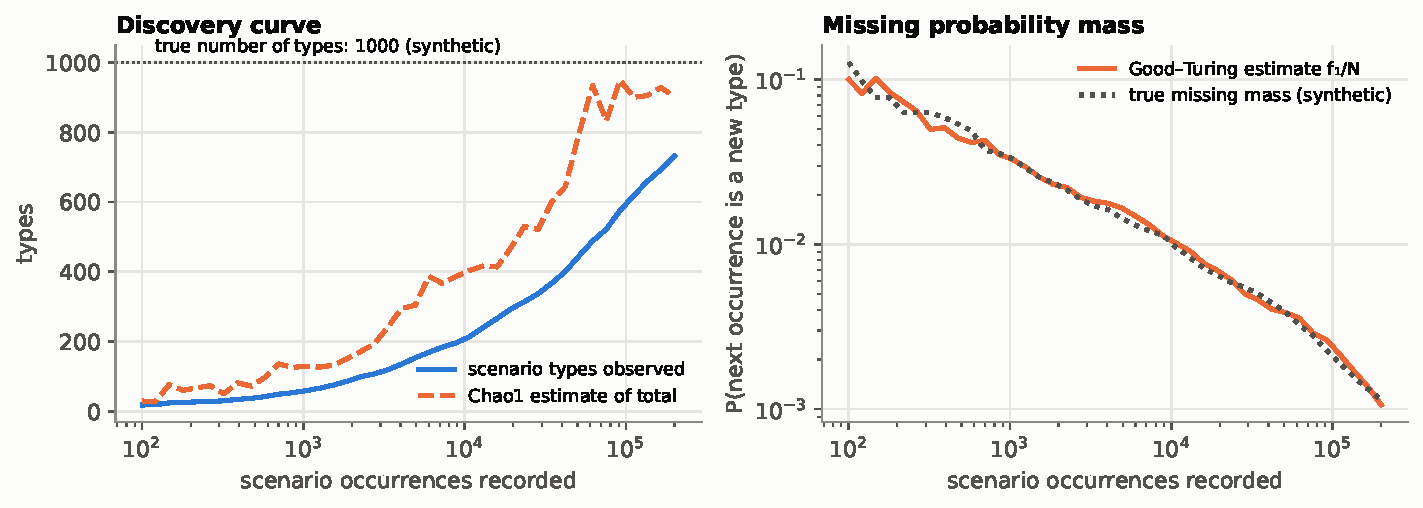
\includegraphics[width=\linewidth]{figures/f26_saturation.pdf}
\caption{Synthetic: 1{,}000 scenario types with Zipf frequencies (exponent 1.8)\synthetic. After 200{,}000 occurrences, 731 types are seen and Chao1 estimates 902, a lower bound; the Good--Turing missing mass is $1.06\times10^{-3}$ (true $1.14\times10^{-3}$) \own{computed}.}
\end{figure}

\subsection{OpenLABEL and ISO 34504}
\begin{table}[H]\centering\small
\caption{ASAM OpenLABEL compared with ISO~34504.}
\begin{tabular}{L{2.4cm}L{6.2cm}L{5.6cm}}
\toprule
& ASAM OpenLABEL 1.0.0 (2021) & ISO 34504:2024\\\midrule
nature & data format (JSON schema) for annotations \cite[standard page]{asamopenlabel} & vocabulary and structure for scenario categories \cite[web article]{tno2024}\\
content & elements (objects, actions, events, contexts, relations) with name, uid, type and ontology id \cite[Sec.~2.3.1]{openlabelconcept}; relations as RDF triples \cite[Sec.~2.3.4]{openlabelconcept}; frames and frame intervals \cite[Secs.~2.3, 2.3.2]{openlabelconcept}; streams \cite[Secs.~2.3, 2.3.6]{openlabelconcept}; coordinate systems \cite[Secs.~2.3.7, 3.1]{openlabelconcept} & tags for vehicle types, environments, light, weather, road conditions, grouped into categories; examples, no exact values \cite[web article]{tno2024}\\
semantics & none of its own: elements point to external ontologies \cite[Secs.~2.3, 2.3.3]{openlabelconcept} & a semantic source to point to\\
scenario tags & labels selected from a pool and stored with scenario files for search \cite[Secs.~5.1--5.2]{openlabelconcept} & tags define the categories\\
related & lists BSI PAS~1883 and ASAM OpenODD \cite[Sec.~1.3]{openlabelconcept} & part of the ISO 3450x family \cite[web article]{tno2024}\\
\bottomrule
\end{tabular}
\end{table}
They complement each other: ISO~34503/34504 plus custom tags form the ontology; OpenLABEL stores per-recording, per-interval annotations that reference it; the scenario database indexes them; OpenSCENARIO describes executable tests.

%=====================================================================
\section{Scaling to ACC and an L4 robotaxi}\label{sec:scaling}
The estimator \eqref{eq:risk} does not change; the scenario space, the agent interaction and the cost of exploring rare regions do.
\begin{table}[H]\centering\small
\caption{Three levels compared \own{assessment}.}
\begin{tabular}{L{2.6cm}L{3.4cm}L{3.8cm}L{4.4cm}}
\toprule
& unintended braking (Sec.~\ref{sec:example}) & ACC / L2 longitudinal & L4 urban robotaxi\\\midrule
hazardous behaviours & 1 & about 5--10 & dozens across all DDT subtasks\\
scenario types & 1 & follow, lead braking, cut-in, cut-out, queue approach & hundreds: intersections, occluded VRUs, pick-up/drop-off, emergency vehicles\\
parameters & 7 & about 10--20 & about 50--100 and more\\
interaction & open loop & closed loop, driver as fallback & closed loop, many reactive agents\\
acceptance & one $A_H$ & per HE, human benchmark (Annex~C) & positive risk balance per harm type (ISO/TS~5083)\\
\bottomrule
\end{tabular}
\end{table}
ACC is specified in ISO~15622 \cite[location not verified]{iso15622}; ISO~21448 uses an ACC lead-braking scenario as its example for parameter distributions and importance sampling \cite[C.5, Figure~C.9, pp.~146--147]{iso21448}. It also warns that the traffic-statistics approach of its AEB example ``can prove impractical'' for a fully automated vehicle ``unless specific considerations with respect to system architecture are made'' \cite[C.2.2.6, p.~134]{iso21448}. With $d$ parameters shifted by $\delta$ standard deviations, a Gaussian proposal gives $E_q[w^2]=e^{d\delta^2}$ and $\mathrm{ESS}/N\approx e^{-d\delta^2}$ \own{derived; Fig.~\ref{fig:ess}}. Fixed-proposal importance sampling therefore degrades in high dimension, which motivates the cross-entropy method \cite[location not verified]{rubinstein2016}, subset simulation \cite[location not verified]{aubeck2001} and adaptive importance sampling \cite[Ch.~10]{owen2013}. Runtime risk models can restrict exposure to risky situations: SINADRA derives monitorable risk-implausibility hypotheses from HARA work products and turns them into Boolean or Bayesian-network runtime models \cite[Sec.~1.3, pp.~4--5; Sec.~4.3, p.~77]{reich2026}; in its urban case study, behaviour-intent likelihoods weight a collision-risk signal \cite[Sec.~5.2.5, p.~131]{reich2026}. Such a reduction of $\nu_\ell$ must be argued inside Eq.~\eqref{eq:risk}.
\begin{figure}[H]\centering
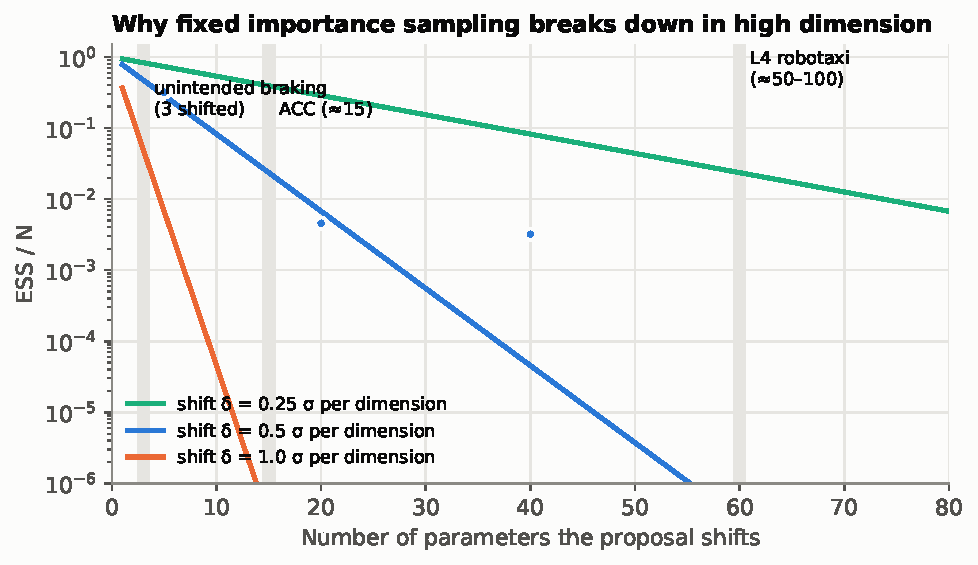
\includegraphics[width=0.86\linewidth]{figures/f22_ess_dim.pdf}
\caption{Effective sample size of importance sampling against the number of shifted parameters \own{derived and simulated}.}
\label{fig:ess}
\end{figure}

%=====================================================================
\section{Equation audit and post-2022 alternatives}\label{sec:audit}
Every equation in this report was checked numerically (script in the repository, \texttt{tools/} and \texttt{report/}): coverage of the zero-failure test by simulation, the Poisson--$\chi^2$ identity for $k=0,\dots,9$, unbiasedness of the importance-sampling estimator and of the copula weights, the copula density against the multivariate normal density, $\rho=\sin(\pi\tau/2)$ by sampling, the TV bound on a test case, $\mathrm{ESS}/N=e^{-d\delta^2}$ by simulation, and the Clopper--Pearson and Jeffreys formulas. Table~\ref{tab:audit} lists the results. ISO~21448 was published in 2022 and its Annex~C methods predate it; the right-hand column names methods published since then.

{\small
\begin{longtable}{L{2.6cm}L{1.6cm}L{5.0cm}L{5.4cm}}
\caption{Equation audit \own{numerical checks} and post-2022 alternatives.}\label{tab:audit}\\
\toprule
Equation & Status & Finding & More recent alternative\\\midrule\endfirsthead
\toprule
Equation & Status & Finding & More recent alternative\\\midrule\endhead
Allocation, Eq.~\eqref{eq:alloc} & \textbf{was wrong, fixed} & $B_j\propto\sqrt{G_j}$ is optimal only for equal $k_j$; with the cells' own $\lambda_{k,j}$ the optimum is $B_j\propto\sqrt{\lambda_{k,j}G_j}$; the old rule needed 567{,}814~h instead of 564{,}084~h \own{computed} & --- \\
Annex~C decomposition, Eq.~\eqref{eq:annexc} & correct under assumptions & exact only with properly conditioned factors; with factors from a different scenario mix a toy case was off by 22\% \own{computed} & estimate per scenario with Eq.~\eqref{eq:risk}; aligned human benchmarks by vehicle type, road type and location \cite[Abstract]{kusano2025} instead of one national statistic as in \cite[C.2.2.4, p.~131]{iso21448}\\
Zero-failure $\tau$, Eq.~\eqref{eq:tau} & correct, incomplete & confidence refers to $\RHB$, not $A_H$, when factors are estimated (Sec.~3.2); fixed sample size, no optional continuation & safe anytime-valid inference: e-processes and confidence sequences allow ``optional stopping or continuation for any reason'' \cite[Abstract]{ramdas2023}; SPRT \cite[Sec.~V]{betschinske2025}\\
$k$-failure plan, Eq.~\eqref{eq:chi2} & correct & verified for $k=0$--9 & same as above\\
Union bound, Eq.~\eqref{eq:bonf}; claim, Eq.~\eqref{eq:claim} & correct, conservative & Bonferroni over 120 terms fails where a joint posterior passes (Sec.~\ref{sec:example}) & Bayesian joint posterior or hierarchical model; Bayesian safety validation with probabilistic surrogates and importance sampling \cite[Abstract]{moss2023}\\
IS estimator and ESS, Eq.~\eqref{eq:is} & correct; ESS misleading & Kish's ESS ignores $h$; in a test case ESS/N was 0.11 while the relative SE was 0.9\%; at $d=15$ the finite-sample ESS overestimated $e^{-d\delta^2}$ by 1.8$\times$ \own{computed} & adaptive, state-dependent IS proposals for sequential systems \cite[Abstract]{delecki2024}; dense RL editing out non-critical states, 10$^3$--10$^5$ times faster evaluation \cite[Abstract]{feng2023}\\
Copula density; $\rho=\sin(\pi\tau/2)$; $t$-copula $\lambda_U$ & correct & verified numerically & vine copulas for high dimension \cite[location not verified]{joe2014}\\
Granularity bound & correct with TV $=\tfrac12L^1$ & definition was missing; now stated & ---\\
Missing mass, Eq.~\eqref{eq:unk} & point estimate & was used like a bound & concentration bound \cite[Theorem~1]{berend2013} (Sec.~\ref{sec:l4})\\
SPI drift detection ($\mu^*\approx 9.1$) & correct & power of the discrete test is not monotone in $\mu$; first crossing used & confidence sequences for continuous monitoring \cite{ramdas2023}\\
Clopper--Pearson, Jeffreys, flat-prior identity & correct & $c=0$, $N=2000$: 7.77/2000 vs.\ $-\ln(1-C_b)=7.78$ & ---\\
\bottomrule
\end{longtable}
}

Field results now report crash rates with confidence intervals against benchmarks aligned to the same vehicle types, road types and locations \cite[Abstract]{kusano2025}, and treat them as ``a directional and continuous confidence growth indicator'' within a safety case \cite[Abstract]{kusano2024}, rather than as a single pass/fail mileage test of the kind in ISO~21448 C.2.2.

%=====================================================================
\section{Limitations}\label{sec:limits}
\begin{itemize}
\item All example data are synthetic; correlations, rates, distributions and the injury curve are illustrative.
\item ISO~21448 references were checked against the standard; ISO/TS~5083, UL~4600, ISO~34502/34503/34504 and ISO~15622 were not available (Sec.~1.2).
\item The kinematic model is one-dimensional, without lateral escape, brake build-up or reaction to brake release.
\item Scenario shares are products of factor shares (independence between trigger, speed and headway).
\item The Bayesian result depends on the prior, which must be defended to an assessor.
\end{itemize}

%=====================================================================
\appendix
\section{Code and reproduction}\label{app:code}
All numbers marked \textit{this report} and all figures are reproducible from the repository \texttt{dfeldmann-bot/sotif-risk-course} (private): \texttt{tools/ub\_sim.py} (scenario generation, copula, simulation, weights), \texttt{tools/build\_ub\_example.py} (workbook with live formulas), \texttt{tools/build\_docs\_html.py} (figures and HTML docs) and \texttt{tools/gen\_report\_figs.py} (the figures of this report). Random seed: 2026.

%=====================================================================
\begingroup\small
\begin{thebibliography}{99}
\bibitem{iso21448} ISO 21448:2022(E). \emph{Road vehicles --- Safety of the intended functionality.} First edition, 2022-06. ISO, Geneva. Page numbers as printed.
\bibitem{iso34502} ISO 34502:2022. \emph{Road vehicles --- Test scenarios for automated driving systems --- Scenario based safety evaluation framework.} ISO.
\bibitem{iso34503} ISO 34503:2023. \emph{Road vehicles --- Test scenarios for automated driving systems --- Specification for operational design domain.} ISO.
\bibitem{iso15622} ISO 15622. \emph{Intelligent transport systems --- Adaptive cruise control systems --- Performance requirements and test procedures.} ISO.
\bibitem{tno2024} TNO (2024). New ISO 34504 provides guidance for safety assessment of automated driving systems. \url{https://www.tno.nl/en/newsroom/insights/2024/05/iso-34504-safety-and-automated-driving/}
\bibitem{asamopenlabel} ASAM e.V. (2021). ASAM OpenLABEL 1.0.0. \url{https://www.asam.net/standards/detail/openlabel/}
\bibitem{openlabelconcept} ASAM e.V. OpenLABEL Concept Paper. \url{https://www.asam.net/fileadmin/Projects/Project-Details/P_2020_12_OpenLABEL_V1.0.0/OpenLABEL_Concept_paper.html}
\bibitem{siemensnatm} Siemens Digital Industries Software. Multi-pillar approach for safety validation of automated vehicles (on UNECE NATM, ECE/TRANS/WP.29/2021/61, and Regulation (EU) 2022/1426). \url{https://blogs.sw.siemens.com/simcenter/multi-pillar-approach-for-safety-validation-of-automated-vehicles/}
\bibitem{putze2023} L.~Putze, L.~Westhofen, T.~Koopmann, E.~Böde, C.~Neurohr (2023). On quantification for SOTIF validation of automated driving systems. arXiv:2304.10170.
\bibitem{betschinske2025} D.~Betschinske, M.~Schrimpf, S.~Peters, K.~Klonecki, J.~P.~Karch, M.~Lippert (2025). Towards more efficient quantitative safety validation of residual risk for assisted and automated driving. arXiv:2506.10363.
\bibitem{kalra2016} N.~Kalra, S.~M.~Paddock (2016). \emph{Driving to Safety: How Many Miles of Driving Would It Take to Demonstrate Autonomous Vehicle Reliability?} RAND Corporation, RR-1478-RC.
\bibitem{schaller2026} F.~Schaller, R.~Ehlers, I.~Aslam, A.~Deshpande, R.~Gräfe, W.~Guedri, N.~Habib, N.~Maslov, A.~Rausch, S.~S.~Qutub, M.~Zhang (2026). Addressing SOTIF with a runtime monitor ensemble for AI-based perception systems. \emph{Discover Artificial Intelligence} 6:1172. doi:10.1007/s44163-026-02186-z.
\bibitem{reich2026} J.~Reich (2026). \emph{SINADRA: Situation-Aware Dynamic Risk Assessment for Safe and Permissive Autonomous Systems.} Dr.-Ing. thesis, RPTU Kaiserslautern-Landau / Fraunhofer IESE. Page numbers as printed.
\bibitem{degelder2022} E.~de Gelder (2022). \emph{Safety assessment of automated vehicles using real-world driving scenarios.} PhD thesis, TU Delft.
\bibitem{degelder2024} E.~de Gelder, M.~Buermann, O.~Op den Camp (2024). Coverage metrics for a scenario database for the scenario-based assessment of automated driving systems. arXiv:2409.01139 (v2).
\bibitem{glasmacher2024} C.~Glasmacher, H.~Weber, L.~Eckstein (2024). Towards a completeness argumentation for scenario concepts. arXiv:2404.01934.
\bibitem{guo2023} D.~Guo, M.~Muñoz Sánchez, E.~de Gelder, T.~P.~J.~van der Sande (2023). Scenario extraction from a large real-world dataset for the assessment of automated vehicles. arXiv:2306.07815.
\bibitem{unsupervised2022} Toward unsupervised test scenario extraction for automated driving systems from urban naturalistic road traffic data. arXiv:2202.06608.
\bibitem{hauer2019} F.~Hauer, T.~Schmidt, B.~Holzmüller, A.~Pretschner (2019). Did we test all scenarios for automated and autonomous driving systems? \emph{IEEE ITSC 2019}.
\bibitem{zhao2017} D.~Zhao, H.~Lam, H.~Peng, S.~Bao, D.~J.~LeBlanc, K.~Nobukawa, C.~S.~Pan (2016). Accelerated evaluation of automated vehicles safety in lane-change scenarios based on importance sampling techniques. arXiv:1605.04965; doi:10.1109/TITS.2016.2582208.
\bibitem{ratiu2024} D.~Ratiu, T.~Rohlinger, T.~Stolte, S.~Wagner (2024). Towards an argument pattern for the use of safety performance indicators. arXiv:2410.00578.
\bibitem{koopman2022} P.~Koopman (2022). Safety Performance Indicators (SPIs) for Autonomous Vehicles. Lecture slides, Carnegie Mellon University. \url{https://users.ece.cmu.edu/~koopman/lectures/L124_SPI_vs_KPI.pdf}
\bibitem{waymoinjury} Waymo. An omni-directional model of injury risk in planar crashes. \url{https://waymo.com/research/an-omni-directional-model-of-injury-risk-in-planar/}
\bibitem{littlewood1997} B.~Littlewood, D.~Wright (1997). Some conservative stopping rules for the operational testing of safety-critical software. \emph{IEEE Transactions on Software Engineering} 23(11):673--683. Source of ISO~21448 Formula~(C.7).
\bibitem{feng2023} S.~Feng, H.~Sun, X.~Yan, H.~Zhu, Z.~Zou, S.~Shen, H.~X.~Liu (2023). Dense reinforcement learning for safety validation of autonomous vehicles. \emph{Nature} 615:620--627. doi:10.1038/s41586-023-05732-2.
\bibitem{kusano2024} K.~D.~Kusano, J.~M.~Scanlon, Y.-H.~Chen, T.~L.~McMurry, R.~Chen, T.~Gode, T.~Victor (2024). Comparison of Waymo rider-only crash data to human benchmarks at 7.1 million miles. \emph{Traffic Injury Prevention}, doi:10.1080/15389588.2024.2380786; arXiv:2312.12675.
\bibitem{kusano2025} K.~D.~Kusano, J.~M.~Scanlon, Y.-H.~Chen, T.~L.~McMurry, T.~Gode, T.~Victor (2025). Comparison of Waymo rider-only crash rates by crash type to human benchmarks at 56.7 million miles. arXiv:2505.01515.
\bibitem{ramdas2023} A.~Ramdas, P.~Grünwald, V.~Vovk, G.~Shafer (2023). Game-theoretic statistics and safe anytime-valid inference. \emph{Statistical Science} 38(4); arXiv:2210.01948.
\bibitem{moss2023} R.~J.~Moss, M.~J.~Kochenderfer, M.~Gariel, A.~Dubois (2023/2024). Bayesian safety validation for failure probability estimation of black-box systems. arXiv:2305.02449; doi:10.2514/1.I011395.
\bibitem{delecki2024} H.~Delecki, S.~M.~Katz, M.~J.~Kochenderfer (2024). Failure probability estimation for black-box autonomous systems using state-dependent importance sampling proposals. arXiv:2412.02154.
\bibitem{berend2013} D.~Berend, A.~Kontorovich (2013). On the concentration of the missing mass. \emph{Electronic Communications in Probability}; arXiv:1210.3248.
\bibitem{mcallester2000} D.~McAllester, R.~E.~Schapire (2000). On the convergence rate of Good--Turing estimators. \emph{COLT 2000}.
\bibitem{joe2014} H.~Joe (2014). \emph{Dependence Modeling with Copulas.} CRC.
\bibitem{garwood1936} F.~Garwood (1936). Fiducial limits for the Poisson distribution. \emph{Biometrika} 28:437--442.
\bibitem{clopper1934} C.~J.~Clopper, E.~S.~Pearson (1934). The use of confidence or fiducial limits illustrated in the case of the binomial. \emph{Biometrika} 26:404--413.
\bibitem{good1953} I.~J.~Good (1953). The population frequencies of species and the estimation of population parameters. \emph{Biometrika} 40:237--264.
\bibitem{chao1984} A.~Chao (1984). Nonparametric estimation of the number of classes in a population. \emph{Scandinavian Journal of Statistics} 11:265--270.
\bibitem{aubeck2001} S.-K.~Au, J.~L.~Beck (2001). Estimation of small failure probabilities in high dimensions by subset simulation. \emph{Probabilistic Engineering Mechanics} 16(4).
\bibitem{lindskog2003} F.~Lindskog, A.~McNeil, U.~Schmock (2003). Kendall's tau for elliptical distributions. In \emph{Credit Risk}, Physica.
\bibitem{embrechts2003} P.~Embrechts, F.~Lindskog, A.~McNeil (2003). Modelling dependence with copulas and applications to risk management. In \emph{Handbook of Heavy Tailed Distributions in Finance}, Elsevier.
\bibitem{owen2013} A.~B.~Owen (2013). \emph{Monte Carlo theory, methods and examples.} Ch.~9 (importance sampling), Ch.~10 (advanced variance reduction). \url{https://artowen.su.domains/mc/}
\bibitem{nelsen2006} R.~B.~Nelsen (2006). \emph{An Introduction to Copulas}, 2nd ed. Springer.
\bibitem{coles2001} S.~Coles (2001). \emph{An Introduction to Statistical Modeling of Extreme Values.} Springer.
\bibitem{rubinstein2016} R.~Y.~Rubinstein, D.~P.~Kroese (2016). \emph{Simulation and the Monte Carlo Method}, 3rd ed. Wiley.
\end{thebibliography}

\subsection*{Further reading: statistics books}
\begin{itemize}
\item L.~Wasserman (2004). \emph{All of Statistics.} Springer. Compact rigorous inference; a good first book.
\item G.~Casella, R.~L.~Berger (2002). \emph{Statistical Inference}, 2nd ed. Duxbury. Estimators, confidence intervals, tests.
\item W.~Q.~Meeker, G.~J.~Hahn, L.~A.~Escobar (2017). \emph{Statistical Intervals}, 2nd ed. Wiley. Exact Poisson and binomial intervals, demonstration tests (chapter not verified).
\item M.~Rausand, A.~Barros, A.~Høyland (2020). \emph{System Reliability Theory}, 3rd ed. Wiley. Failure rates and Bayesian reliability (chapter not verified).
\item A.~Gelman et al.\ (2013). \emph{Bayesian Data Analysis}, 3rd ed. CRC. Priors and posteriors; Ch.~2 single-parameter models including the Poisson model. Free PDF: \url{https://sites.stat.columbia.edu/gelman/book}
\item A.~B.~Owen (2013), see \cite{owen2013}: Ch.~9 for importance sampling diagnostics and effective sample size.
\item C.~P.~Robert, G.~Casella (2004). \emph{Monte Carlo Statistical Methods}, 2nd ed. Springer.
\item R.~Y.~Rubinstein, D.~P.~Kroese (2016), see \cite{rubinstein2016}: rare events and the cross-entropy method.
\item R.~B.~Nelsen (2006), see \cite{nelsen2006}: Sec.~2.3 Sklar's theorem; Ch.~5 dependence and Kendall's $\tau$.
\item H.~Joe (2014). \emph{Dependence Modeling with Copulas.} CRC. Vine copulas (chapter not verified).
\item S.~Coles (2001), see \cite{coles2001}: Ch.~4 threshold models and the generalised Pareto distribution.
\end{itemize}
\endgroup
\end{document}
